\documentclass[12pt,a4paper]{article}

\usepackage{graphicx} % Required for inserting images
\usepackage[margin=25mm]{geometry}
\parskip 4.2pt  % Set spacing between paragraphs
\parindent 8.4pt  % Set leading space for paragraphs
\usepackage[font=sf]{caption} % Change font of captions
\usepackage{tocloft} % Reduce table of contents line spacing
\usepackage{enumitem}
\usepackage{amsmath}
\usepackage{amsfonts}
\usepackage{amssymb}
\usepackage{siunitx}
\usepackage{verbatim}
\usepackage{hyperref} % Required for inserting clickable links
\usepackage{natbib} % Required for APA-style citations
\usepackage{comment}
\usepackage{wrapfig}
\usepackage{xcolor}

\definecolor{materialgreen}{RGB}{76, 175, 80}
\newcommand{\notetp}[1]
	{{\color{materialgreen}[[{\bf Thomas:} #1]]}}

\title
{
    \textbf{CPSC436A Final Report}
    \\
    \large{\textbf{Filling Barrelfish with Chum}}
}
\author
{
    {\rm Adrian Pikor}\\\textit{University of British Columbia}
    \and
    {\rm Arya Stevinson}\\\textit{University of British Columbia}
    \and
    {\rm Linh Pham}\\\textit{University of British Columbia}
    \and
    {\rm Mathew Balsdon}\\\textit{University of British Columbia}
}

\begin{document}
\captionsetup[figure]{skip=0pt}
\maketitle
\newpage

\tableofcontents
\newpage

\section{Introduction}
Operating systems are a long and historied part of computer science whose importance is hard to downplay. They serve as the backbone for all modern computing systems and play a crucial role in managing tasks such as process scheduling, memory allocation, and device communication. The significance of such a system lies in its ability to abstract away hardware complexities and ensure seamless, secure, and efficient interaction between users and the underlying computer hardware.
\\\\
Barrelfish is a research operating system that distinguishes itself by way of its unique design philosophy and innovative architecture. Unlike traditional monolithic or microkernel-based systems, Barrelfish employs a distributed multikernel approach which aims to maximize the potential of the modern multicore and multiprocessor systems over which it lies. In this paper we describe how our group designed and implemented a few of its key subsystems including physical memory management, paging, inter-process communication, and more.

\subsection{Team Structure}
The development process as an individual is relatively straightforward but often not fast enough in order to adhere to tight deadlines and larger project specifications. For this class, both factors were at play and so teamwork was necessary. We organized into a group of four and promptly discussed how work should be split up.
\\\\
Progress in the class was divided into ``Milestones" which denoted the completion of large overarching pieces of the operating system. These were further divided up into ``functionalities" that described finer-grained and sometimes parallelizable tasks which made up the whole of the Milestone. At the end of each Milestone deadline, groups were required to give a presentation on what they were able to do and how they did it. It should also be noted that on the turn of each deadline, every group member was expected to understand every part of the implemented code for that Milestone.
\\\\
Given the task/deadline structure and because we were a small group of students with oftentimes chaotic schedules, the only way by which we could significantly split work was through having one person work on code sections at a time so as to prevent merge conflicts. Allocation of work was more often than not based on who had the time for it, with individual members opting to pick up free tasks wherever possible. We also observed a rather emergent development pattern where if two members were free at the same time they would share ideas and talk through tasks with each other which we believe significantly sped up the process (in other words, a sort of online pair programming where one member was actively coding and the other was checking in to help with roadblocks). We recognize that having members opt in to tasks is not the most robust team structure since a bad actor could always simply decide to not do anything, however this is and has always been a sort of inevitability of school group projects due to a lack of any external incentives (such as getting fired).

\subsection{Tools}
Our team primarily used Discord for communication when face-to-face meetings were not possible and Git/GitHub for version control. Initially we decided to use GitHub's built in ``Project Boards" feature to keep track of, allocate, and manage tasks, however this quickly fell out of favor since the group was small enough such that we were all able to easily keep up-to-date on tasks without the use of it.

\newpage

\section{Memory Management}
Before we can start doing anything interesting with our operating system, we need a framework for managing physical memory, since it serves as the backbone of many other OS functions. Physical memory management is done through a structure called the ``memory manager".

\subsection{Capabilities}
Capabilities can be thought of as keys to a door. Under the classical ``access-control" approach to operating systems, different sections of memory are associated with a list of users who have various rights with respect to that section of memory; for example, a file \textbf{F} that can be read from by processes \textbf{A} and \textbf{B}. In contrast, capabilities define a list of memory sections that they have rights to. In terms of our access-control example, processes \textbf{A} and \textbf{B} would instead hold a capability to the file \textbf{F} that allows them to various abilities (read/write/execute) to it. Oftentimes in this paper we will also refer to the ``CSpace", which can simply be thought of as a process' storage for its capabilities. The CSpace is structured as a two-level table that only the kernel may directly modify. When we refer to capabilities in later sections of this report, we really mean a \textit{reference} to the capability, as our user-level processes do not directly manage the capabilities. 

\subsection{Design Constraints}\label{m1-0}
At this stage in our operating system, we have a single, privileged process running, called \texttt{init}. This process has been handed several capabilities to different portions of RAM and we must devise a method through which we can divide and distribute these portions on request. We encapsulate the data structure and algorithm that will perform this task in a ``physical memory manager". From this point forward in our OS, any and all physical memory allocations/frees are performed by this memory manager. Although this memory manager is meant to provide RAM resources to the entire system, as we mentioned earlier, we only have one core running a single process with a single thread. As such, the following sections describe an implementation that does not handle concurrency.
\\\\
The memory manager must keep track of all allocated and free physical memory, otherwise we would not have any way to tell what is and isn't currently being used. When a process requests memory, the memory manager must locate an appropriate section of free physical memory and provide a RAM capability to the caller. RAM capabilities can be understood as just that; capabilities to sections of RAM. They may be retyped into a variety of more fine-grained capabilities (denoting more specific things one might do with the memory that the capability points to), and they also may be passed between processes (the fundamental mechanism by which our memory manager distributes memory).
\\\\
There are two big decisions that need to be made when implementing the memory manager:
\begin{enumerate}[itemsep=0pt]
    \item What data structure should we be using to represent the physical address space? 
    \item Given that we don't know what allocations and frees will happen ahead of time, how do we decide which parts of the physical address space to allocate?
\end{enumerate}
Just as it is when setting out to design any operating system, it was necessary that our group give a lot of thought to these questions as it would have a direct impact on the efficiency of our system in both speed and fragmentation. On that note, however, it should also be mentioned that deadline pressure was a very real factor in the decisions we made; while it would be nice to sit around all day and conjure up hyperefficient implementations of Barrelfish, we sometimes simply didn't have the time to do so. The existence of tight deadlines introduced a few external considerations to our design choices:
\begin{itemize}[itemsep=0pt]
    \item We should reuse code where possible (and reasonable). This saves time in that the code is already verified and doesn't need to be written from the ground up.
    \item Designs should not be overly complicated. Complexity often makes systems more error-prone and causes those errors to take longer to understand/debug.
\end{itemize}
This was especially prevalent for our group considering that we are all full-time students with very different and often clashing schedules. It should become clear over time that these were often some of if not the defining factors in our design decisions.

\subsection{Physical Memory Layout}\label{m1-3}
As mentioned previously, we needed to choose a data structure to maintain metadata regarding the free and allocated regions of physical address space. We also needed our structure to be able to locate appropriate sections of memory to satisfy allocation requests as well as update metadata when regions become free. There were a few considerations that we took into account when choosing such a structure for the memory manager:
\begin{itemize}[itemsep=0pt]
    \item Our data structure should take up an acceptable amount of memory.
    \item We should be able to perform efficient searches through our data structure for given address regions.
    \item We should be able to perform efficient insertions/deletions of address regions using our data structure. We would also ideally like for these operations to not negatively effect subsequent searches through the data structure.
    \item The implementation of our data structure should not be too complex due to the time constraints.
\end{itemize}

\subsubsection{Linked List}\label{m1-2}
We chose to use a linked list to maintain the memory manager's metadata, based on the fact that it provided an acceptable solution with respect to our previous considerations:
\begin{itemize}
    \item A linked list allows us to represent memory regions of arbitrary size and number.
    \item A linked list sacrifices efficient traversal of its nodes for a straightforward, linear-time walk of the list in search for an allocated or free address region. Due to our time constraints, a less complex data structure traversal was of higher value than improved efficiency.
    \item By storing pointers to the next and previous node in the linked list, we can easily insert new nodes or remove nodes at a specific position in our linked list, preserving the order of our list. Although the ordering of nodes in our list is not too important for the physical memory manager, it will play a factor later on in Milestone 2.
\end{itemize}
Nodes of the list represent regions of physical memory and can be either free or allocated. The list contains nodes representing the entire, free address space at the beginning of time. Subsequent operations (such as allocation of a region) split and/or coalesce nodes accordingly. Since nodes represent regions, they also need to store info such as their base address and size. 

\subsection{Allocation Strategy}
An allocation strategy determines which memory region the memory manager chooses to satisfy an allocation request. A good allocation strategy minimizes allocation latency and minimizes fragmentation of the physical address space for an average workload. By ``minimizes fragmentation", we mean that if we have a total X bytes of free memory, ideally we would like to be able to allocate X bytes of memory. In practice however this is nearly never the case due to arbitrary allocation sizes and arbitrary routines of allocations and frees.

\subsubsection{Next Fit}
Out of the memory manager functions we wrote, of particular note is \texttt{choose\_region} which decides what part of the address space to allocate when serving a request. We decided to go with a \texttt{next-fit} strategy here, which chooses the first region suitable for an allocation (it must be free and large enough) and begins its search at the region following whichever one was most previously allocated. For this to work, the memory manager is required to store a pointer to its most recently allocated region and a bit of complexity needs to be added to the algorithm (as compared to something like \texttt{first-fit}), however we decided to go with it nonetheless due to its benefit as a ``jack-of-all-trades" approach.

\subsubsection{Alternative Strategies}
We provide a comparison of \texttt{first-fit}, \texttt{worst-fit}, \texttt{best-fit}, and \texttt{next-fit} (anything more complicated was not considered due to time constraints):
\begin{itemize}[itemsep=-5pt]
    \item \texttt{first-fit}:
    \begin{itemize}[itemsep=0pt]
        \item Simple to implement
        \item Fragments early addresses significantly since we always start at the beginning
        \item Slows down over time as longer walks of the linked list are required
    \end{itemize}
    \item \texttt{worst-fit}:
    \begin{itemize}[itemsep=0pt]
        \item Low fragmentation; keeps large free regions large
        \item Slow, since a full walk is always necessary
    \end{itemize}
    \item \texttt{best-fit}:
    \begin{itemize}[itemsep=0pt]
        \item Minimizes external fragmentation
        \item Slow, since a full walk is always necessary 
    \end{itemize}
    \item \texttt{next-fit}:
    \begin{itemize}[itemsep=0pt]
        \item Reasonable fragmentation (spreads allocations across the space)
        \item Reasonably fast; searches finish quicker since we remember where we stopped
    \end{itemize}
\end{itemize}
We compared \texttt{first-fit} and \texttt{next-fit} in the case of many subsequent allocations without any frees (Figure \ref{figure:mm_alloc_scatter}) and found that both appear to demonstrate linear growth in latency with respect to the number of allocated regions, however \texttt{next-fit} grows more slowly. Upon choosing an appropriate RAM capability, the memory manager must split and retype it to return to the requesting process. Retyping a capability must be handled with care, so as to not fall into a case where a region of physical memory is referred to by capabilities of conflicting types, and thus require walking of the process's CSpace to check for descendants or siblings of the capability. Due to this retyping operation, which approximately requires linear time, it is not possible to have sub-linear growth in either \texttt{first-fit} or \texttt{next-fit}. Note that there appears to be a second, lower-density line of higher-latency points; these likely correspond to allocations that triggered slab/slot allocator refills (detailed in the next section).
\begin{figure}[ht]
    \centering
    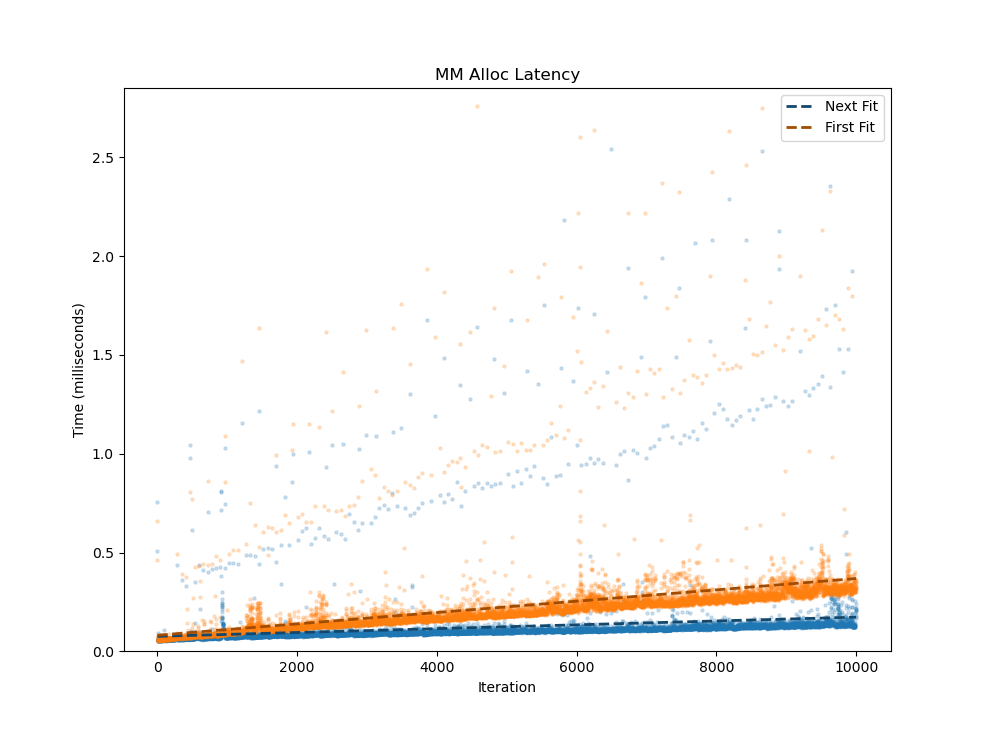
\includegraphics[width=\columnwidth]{images/mm_alloc_scatter.png}
    \caption{Allocation latencies for different strategies.}
    \label{figure:mm_alloc_scatter}
\end{figure}

\subsection{Allocator Refills}
Since the memory manager cannot dynamically allocate memory to store data in, it uses ``slab allocators" to partition memory into small chunks for storage of its metadata nodes. It also uses a ``slot allocator" which allocates capability slots from the CSpace such that the memory manager can store new retyped capabilities (remember, capabilities themselves take up memory). Both of these allocators occasionally require memory refills which are served by the memory manager.
\\\\
To prevent an infinite loop of allocator refills, we set a \texttt{refill} flag whenever an allocator initiates a refill. Until the flag is cleared, no refills are to be triggered. To ensure that there are enough remaining resources to fully complete a refill request, slot and slab allocators have a respective thresholds. When the number of slots/slabs dips below the threshold, a refill is triggered. 

\subsection{Alternative Memory Manager Designs}\label{m1-6}
A disadvantage of linked lists is that finding a particular region takes time $O(n)$ for $n$ nodes. This is particularly relevant when freeing a region, since it first needs to be located in the list.
\\\\
We considered a few alternative data structures:
\begin{itemize}[itemsep=0pt]
        \item \texttt{Static array}: This looks good at first glance on basis of lookups and insertions being constant-time, however using a static array would either severely limit the number of possible allocations, or introduce a massive memory overhead.
        \item \texttt{Balanced tree}: A more complex data structure such as a balanced binary search tree might provide faster lookup times. If the tree is sorted by address, it would allow freeing a region in $O(logn)$ rather than the $O(n)$ for a linked list. Depending on the allocation strategy, the tree might better be sorted by region size which would support a fast implementation of best-fit or worst-fit. However, more complex data structures are also most prone to errors. Since bugs in the memory manager could severely impact all other aspects of the system, we chose to avoid a complex implementation like this. 
\end{itemize}

\subsection{Partial Frees}
We chose to implement partial frees, allowing a procedure to free only a subset of an originally allocated address region. Luckily, the linked-list data structure allowed us to implement this easily through splitting of an allocated region's node in the linked list and marking only the requested segment as free.

\subsection{Ranged Allocation}
We also chose to implement ranged allocations, allowing procedures to make allocation requests within a specified region of physical addresses. Since the linked list maintains address order it also wasn't too tough to implement this; we walk the list and search for any regions containing addresses within the requested range which have a sufficient size. If one is found it can be split appropriately and only the requested region will be marked as allocated.

\newpage

\section{Virtual Memory System}\label{M2}
In Milestone 1, user-space processes were given the ability to obtain physical memory through the capabilities system, and we also implemented a bare-bones virtual address space that could handle very simple mappings. In order to do things like spawn a process (which we do in Milestone 3), we require a full virtual memory system supporting arbitrary mappings and unmappings as well as an MMU-independent, per-process paging system.

\subsection{Design Constraints}
As mentioned above, our user-space processes can now obtain RAM capabilities and retype them into frames. To actually use this memory though, they need to be able to map the frames to virtual addresses. In other words, we want our processes to each be able to use the entire memory space without having to worry about what parts of it are in use by other processes. This implies that we need a mechanism for translating between process memory and actual physical memory (hence why we say ``map physical frames to virtual addresses"). This provides us with a number of benefits such as being able to avoid allocating large chunks of physical memory until necessary, as well as being able to load programs at arbitrary physical locations (even though they were compiled and linked for specific addresses).
\\\\
It is conventionally the job of the MMU to deal with virtual address translation, however since our OS is self-paging, processes explicitly acquire physical memory and then program the MMU with their own constructed page tables. Two main challenges were apparent to our group when we started thinking about a plan of attack for this Milestone:
\begin{enumerate}[itemsep=0pt]
    \item How do we find a free virtual address region to map into? In other words, what per-region metadata needs to be stored and how do we store it?
    \item We need to create page tables for allocated virtual memory space and keep track of their state; how should this be done?
\end{enumerate}
While also fundamental to getting things working, these questions were of particular importance to us since mapping/unmapping operations can easily happen tens of thousands of times during the runtime of an operating system. As such, we were looking for a design that lent itself to quick virtual address region lookups and quick page table lookups/insertions. 

\subsection{Virtual Address Region Layout}
We now describe the first major challenge of this milestone: given a frame, how does a process find an appropriately-sized, free virtual address region to map it to? We need a data structure to maintain the state of virtual address regions. Each region can be free, allocated but not mapped, or allocated and mapped. Some regions will be mapped and physically allocated all at once, e.g. ``eagerly allocated". A region that is virtually allocated but neither mapped nor physically allocated is ``lazily allocated." If a process tries to access the lazily allocated region, a page fault will be triggered and a page of physical memory will be mapped to back the virtual address. In following sections, we will sometimes denote virtual memory allocation as ``reservation" to provide lexical distinction between virtual and physical memory allocation. For this section, we focus on the ``virtual memory manager", which maintains metadata for virtual address regions and determines which regions to allocate on request. Since this problem is almost identical to that of physical memory management in Milestone 1, we must consider the same data structure requirements as we did for the \hyperref[m1-3]{physical memory manager}. In addition to those listed in the referred section, there is an extra detail to account for in virtual memory management:
\begin{itemize}[itemsep=0pt]
    \item Our data structure should be able to represent non-contiguous virtual address ranges (and mark those range as free/allocated).
\end{itemize}

In Milestone 1, physical addresses were not important to physical memory allocation, as processes do not access memory by physical addresses. This is a different case for our virtual memory manager, where we must consider a memory region's address, in addition to its size.

\subsubsection{The Generic Allocator}\label{m2-2}
We started implementing our virtual region memory manager with a simple linked list, just to get things working (we ended up not having the time to swap this out). Each node in the list would represent a reserved region and store data such as its address, size, and whether or not it was mapped. As we have mentioned, since this problem is almost identical to the issue of physical memory management in Milestone 1, we created an interface for our memory manager structures, which we refer to as the ``generic allocator" to reuse some pre-existing functionality.
\\\\
The generic allocator (shown in Figure \ref{figure:m2_diagram}) is an abstract interface that stores a linked list whose nodes each refer to regions of the address space. As an abstract interface, it allows users to add allocator-specific data for regions, errors, functions, and its backing slab allocator. We take advantage of this feature in our virtual memory manager to store extra region data to distinguish between ``reserved" and ``mapped" memory, which we describe in a later section on \hyperref[m2-4]{Heap Memory Management}. 
\\\\
Code for the generic allocator can be found in \texttt{lib/aos/generic\_allocator.c}.
\begin{figure}[ht]
    \centering
    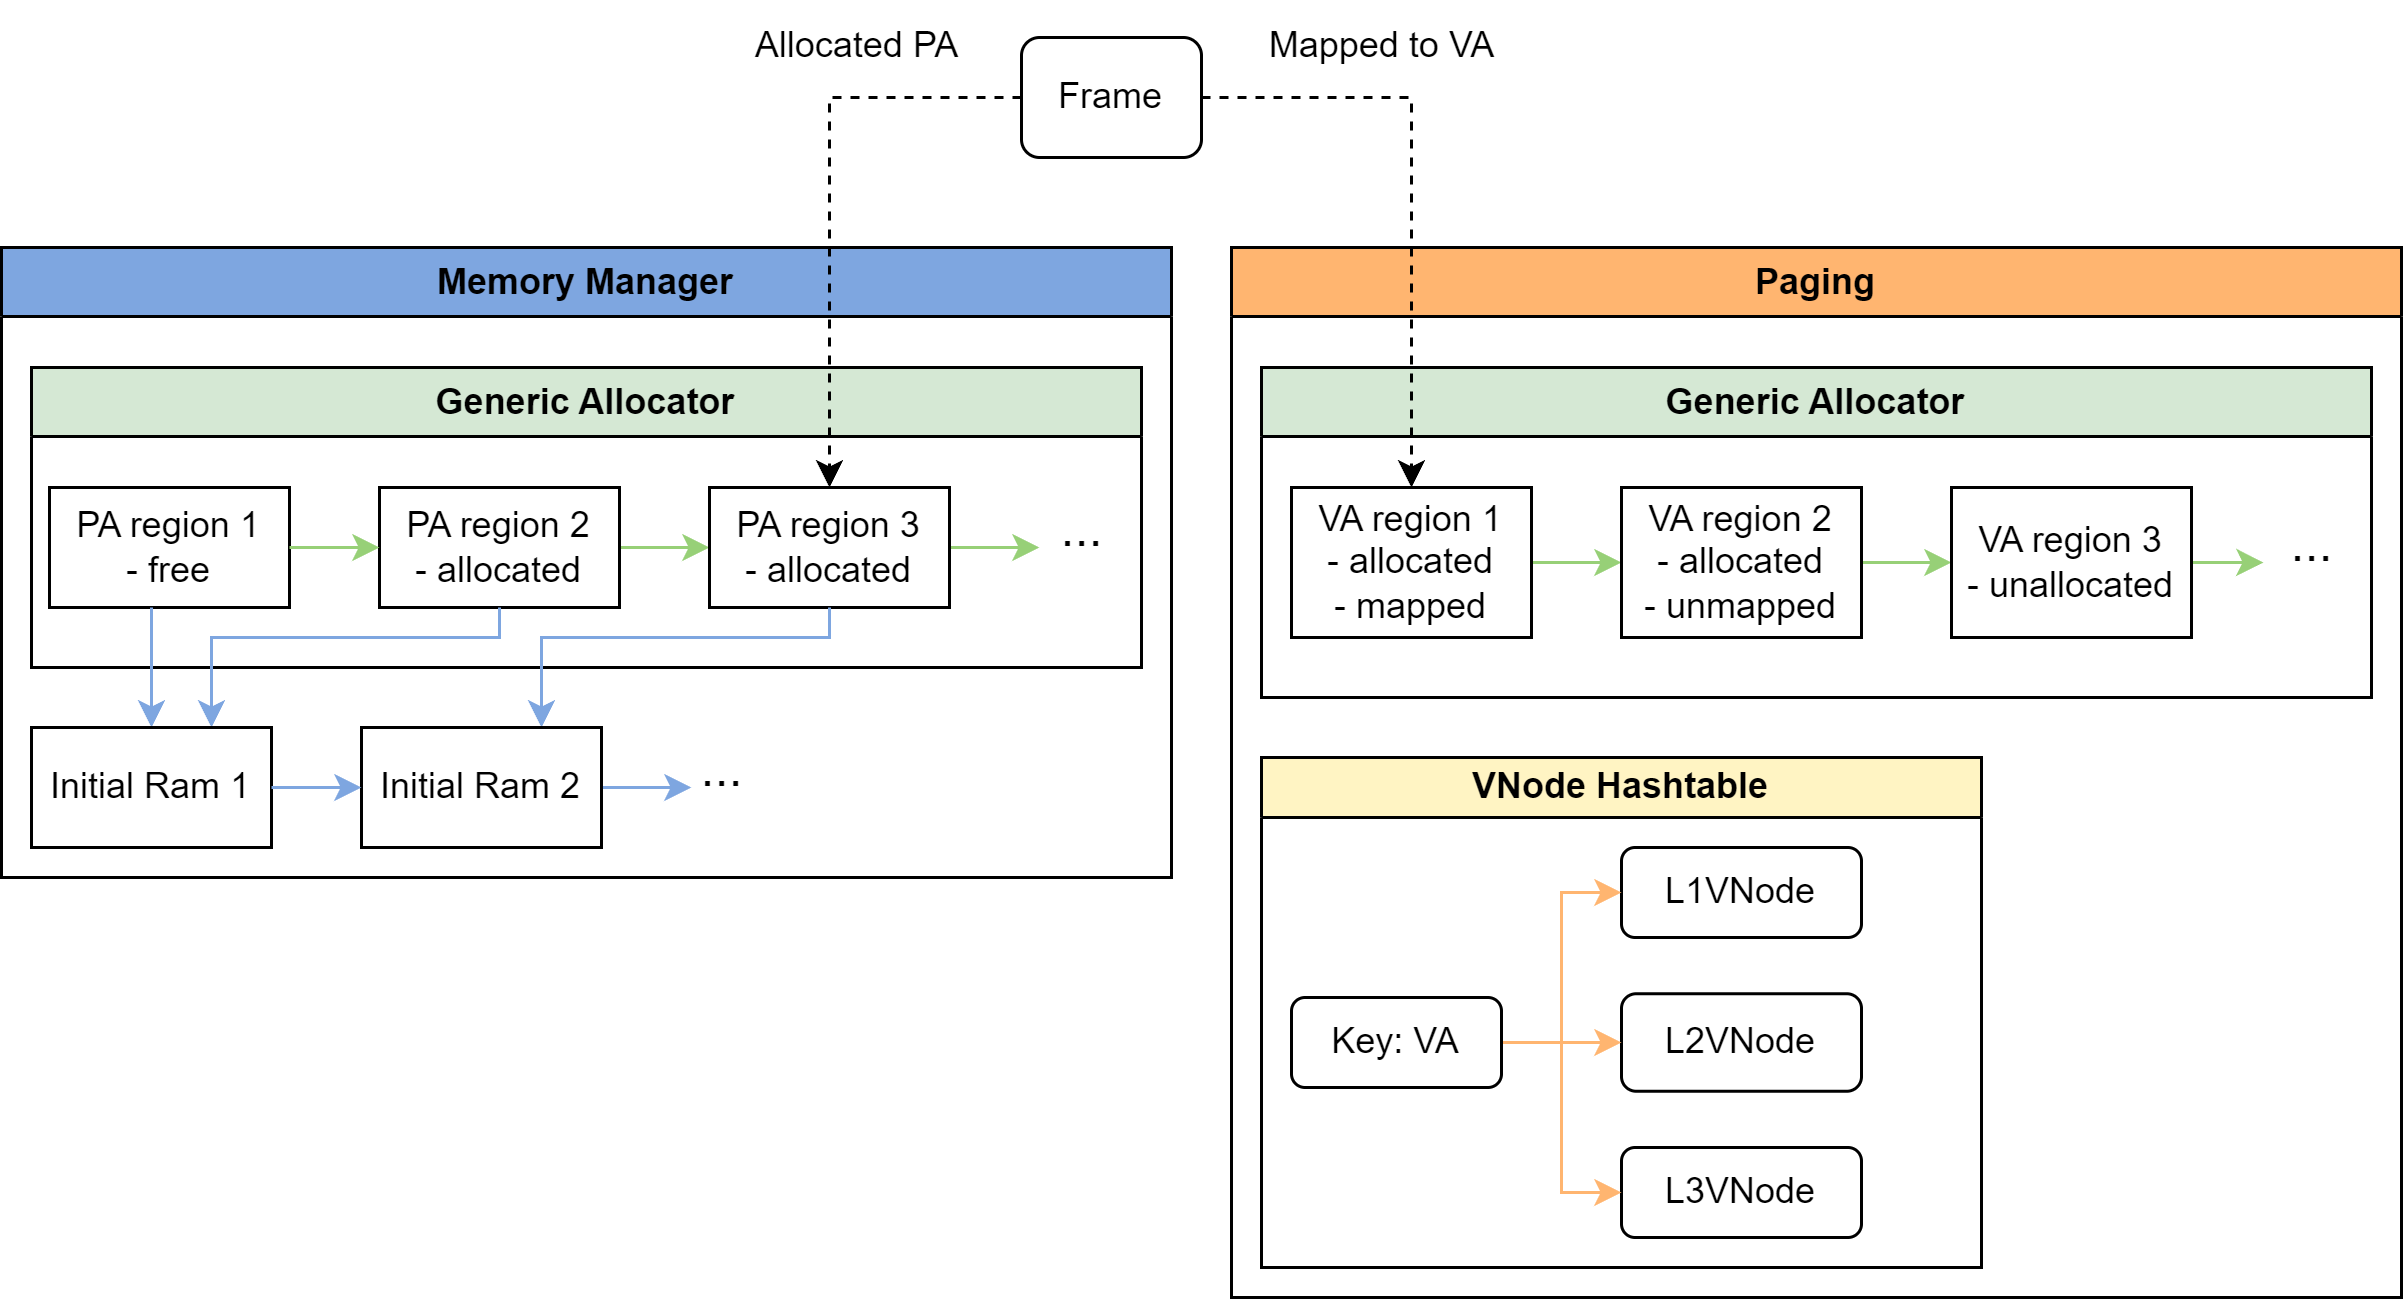
\includegraphics[width=0.8\columnwidth]{images/m2_diagram.png}
    \caption{Usage of the generic allocator in our memory manager and paging implementations.}
    \label{figure:m2_diagram}
\end{figure}
\\\\
The decision to use a linked list, and in particular a ``generic" linked list has been already detailed in \hyperref[m1-2]{Section 2.3.1}. Besides the reasons already described there, the primary benefit of a linked list for the virtual memory manager lies in the fact that a linked list node can easily represent an address range. By storing the starting address and corresponding size of the region in a node, we only require as many nodes as there are allocated regions in our virtual address space, which minimizes the memory overhead by a large margin. In the third point of \hyperref[m1-2]{Section 2.3.1}, we mention that our linked list preserves ordering of the nodes by its base virtual address. This is important to our \texttt{next-fit} allocation strategy, specific to the virtual memory manager. Since we are now concerned with a memory region's addressing during allocation, we do not want an out-of-order list, as \texttt{next-fit} may end up having to walk the entire list in search for an appropriate virtual address to allocate.
\\\\
The alternative data structures detailed in \hyperref[m1-6]{Section 2.6} were also considered for the virtual memory manager and not chosen for the same reasons.
An additional alternative data structure we considered for the task of virtual address region management was a hash table. Using a hash table to represent allocated regions would benefit the implementation with constant-time lookups and insertions as well as less memory usage compared to a static array (on average). However, the primary issue with a hash table is that we cannot easily represent ranges of virtual addresses with \texttt{key:value} pairs. For instance, if we wanted to allocate a 4KiB region at the address \texttt{0xa0000000000} we might naively store the metadata related to the region in the table at the key \texttt{0xa0000000000}, however what happens when we try to check whether the address \texttt{0xa00000008c0} is allocated? This is still within our allocated region however it is not a key within our table, thus it would incorrectly be determined as a free region.

\subsection{Page Table Management}
Once we have decided on a virtual region at which to map a frame (create a translation to the corresponding physical region), we encounter the second main challenge of this Milestone. We need to search for the corresponding page tables (and possibly create them if they don't exist). Reiterating what was mentioned earlier, our OS is self-paging which means processes need to store and handle their own page tables which are then handed off to the MMU.

\subsubsection{Hash Tables}
Although we've dedicated more than a few sentences to our ``simple design first" strategy in previous sections, we decided to achieve this goal using a hash table. The hash table we use has the sole purpose of storing page table metadata. A hash table for the purpose of \textit{page table management} does not suffer from the same issue we outlined in the previous section, where it would not correctly function for \textit{virtual address region management}. The ``address" of a page table, which is the the virtual address up to the page table's index in its upper-level page table, is fixed for virtual addresses within the page table's range. As such, we can set this as the key for the hash table, and ranges of virtual addresses belonging to the same page table will still result in the same page table key.
The hash table key we specifically use is comprised of this page table ``address" and its table level (1, 2, or 3). Take for instance the virtual address \texttt{0xb00008d9000}. The key to the L3 page table for this address would be \texttt{(0xb00008d9000 >> 21) | (3 << 48) = 0x3000000580004}. We shift the virtual address by the number of offset bits used in its parent table (in this example, the L2 index) and then indicate its current level (L3 here) in the higher, unused bits of the virtual address. A subsequent hash table access using this key provides a structure containing page table metadata such as the page table's capability and corresponding mapping capability.
\\\\
Not having gone completely astray from our strategy of keeping things simple, we implemented our hash table by adapting one that was already provided in the initial code handout \cite{bfsource}. Naturally, this implementation had to be changed to use 8-byte integer keys and to allocate memory for entries using a slab allocator (since dynamically allocated heap memory relies on fully functional self-paging, we cannot simply use our friend \texttt{malloc}). The hashing algorithm we used came from a Stack Overflow answer \cite{stackoverflowht}.
\\\\
There were a few difficulties in adapting the hash table for our purposes, namely when mapping cycles occur during the refill of the table's slab allocator. The hash table implementation introduced additional complexity to page table allocation wherein mapping requests that required a page table allocation triggered a slab refill which in turn required the same page table to be allocated. Slab refills must be completed before the frame is mapped as it requires slabs to do so. This caused duplicate insertions into the hash table: the slab refill would allocate a page table that is required by the original request. Upon completing the refill, the original request would try to allocate the same page table---not knowing that the refill has already allocated it. To work around this we decided to define and allocate a specific region of virtual address space to be used only by slab allocators (and thus at which no user-given frames could be mapped to).

\subsubsection{Postmortem}
The idea to use a hash table arose in response to concerns of runtime efficiencies for mapping/unmapping operations when using a linked list. Recall that during mapping/unmapping of a frame, we must initially search for a virtual address region within our virtual memory manager. We then must additionally search for the virtual address's corresponding page tables to perform the mapping/unmapping. As mentioned in \hyperref[m2-2]{Section 3.2.1}, we cannot easily store address ranges (representing allocated/free regions) using a hash table, and thus resorted to using a linked list. Consequently, the first search during mapping/unmapping, for a virtual address region, is relatively slow.
\\\\
This then led to the question of whether we could optimize the runtime of the second search required during a mapping/unmapping operation---for the virtual address's page tables. We figured we could do quick lookups for pre-existing tables by using a hash table since many virtual addresses can be bit-shifted into a per-page-table unique key. Furthermore, once functions for the hash table are implemented, certain operations such as location and insertion of page tables become trivial in code. You may have already noticed a major flaw in this line of reasoning, but at the time, we were, unfortunately, too excited by the prospect of optimization to consider this question more carefully. 
\begin{wrapfigure}{r}{0.5\textwidth}
    \centering
    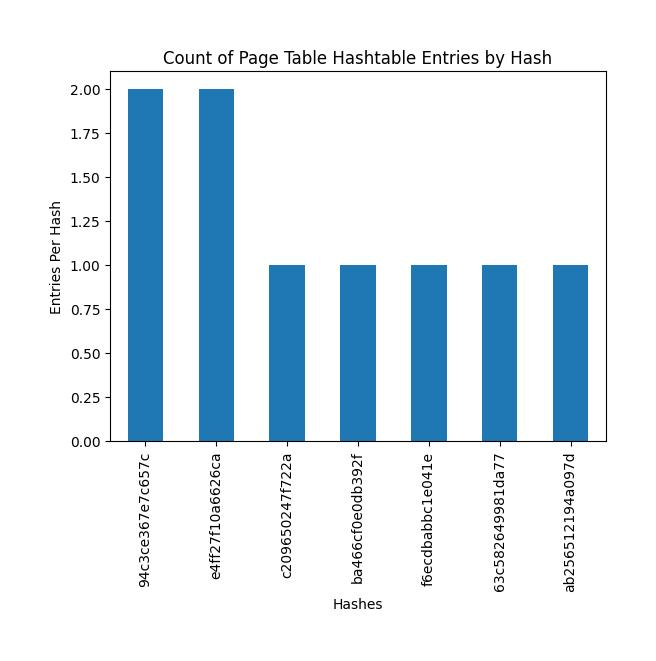
\includegraphics[width=0.5\textwidth]{images/m2_histogram.jpg}
    \caption{Hash table distribution.}
    \label{figure:m2_histogram}
\end{wrapfigure}
\\\\
We painfully recognize in hindsight that using a hash table as an ``optimization" for the overall search-time during a mapping/unmapping operation may not have been as fruitful as we anticipated, due to the sparsity of a process' virtual address space. It is generally the case that large portions of a process's virtual address space, at any given time, don't actually contain data that needs to be stored or processed. This was observed after running one of our test cases which mapped 1,000 arbitrary frames. Although our hash table's distribution was good (Figure \ref{figure:m2_histogram}), it contained only six entries following the mappings. If we had alternatively just stored page tables in a linked list, the search for a free virtual address region would remain the dominating contributor to speed. Put another way, when mapping frames we always must perform a relatively slow search through the linked list of regions in order to find a free space. The overall runtime of a mapping request would not be significantly reduced in the process of searching through an additional few page table nodes stored in a separate linked list. Going with a simpler implementation here would certainly have saved us a few headaches and we figured that we should have more carefully considered whether or not our optimization strategy would have had an observable effect. 

\subsection{Heap Memory Management}\label{m2-4}
In order for processes to freely allocate variable-sized portions of memory, we need to provide a mechanism through which it can access its heap. This is done primarily through a lazy allocation/mapping strategy which is orchestrated through the page fault handler.
\\\\
When a process requests memory from a system that is using lazy allocation, the entire virtual address region is reserved. However, the physical memory allocation and its mapping to any part of that reserved virtual region is only done when the memory is actually accessed. This has a few benefits, for example:
\begin{itemize}[itemsep=0pt]
    \item \textbf{More efficient memory usage}: Physical memory resources are allocated only at the last possible moment, preventing unnecessary allocations of large physical memory blocks that might never be fully used.
    \item \textbf{Reduced initial overhead}: The costs of physical memory allocation and mapping are deferred until later, which is especially helpful in cases where the memory requirements of the requesting process are not initially known.
    \item \textbf{Quicker process spawns}: Lazy allocation makes it unnecessary for a process to physically back all of its heap memory on startup, improving the spawn time.
    \item \textbf{Support for sparsity}: Applications that request large physical chunks of memory, but only use small portions of it are better handled.
\end{itemize}
In order to implement this, we define a specific region of a process's virtual address space as the heap. The page fault handler can only map within this region, and any physical frame that does not make up parts of the heap are not mapped by the fault handler. This introduces the assumption that the only lazily allocated memory is the heap. If we do not make this assumption, then we would need further mechanisms to determine what addresses the page fault handler is allowed to map and to distinguish between addresses belonging to the heap and to other memory regions.
\\\\
As described previously, our virtual memory allocator, in addition to the basic fields provided by its generic interface, distinguishes between ``reserved" and ``mapped" regions. Every mapping is associated with a mapping capability and thus we indicate whether or not a region is mapped by whether or not it holds one or more non-\texttt{NULL} mapping capabilities.
\\\\
When a process tries to access unmapped memory in the heap, a page fault is raised, where control is then handed over to the page fault handler which validates the source of the fault. This includes checking if the accessed address lies within the heap, if the access type is appropriate (read, write, or execute), whether or not we're dereferencing a \texttt{NULL} pointer, and so on. Once the page fault is verified to be a valid virtual memory access, we allocate a page of physical RAM and map it to a page-aligned address containing the faulting address. 

\subsection{Performance Measurements}
Timing measurements were done using the \texttt{time} system call from \texttt{time.h} and then exported and plotted using \texttt{matplotlib}.
\begin{itemize}[itemsep=0pt]
    \item \textbf{Figure \ref{figure:paging_map_small_frame_scatter}}: We evaluated the latency of mapping a series of small frames (1 page each). The average latency increases by only a small margin. Note that there is a second, less dense band of slower latencies above the main band. We suspect that these cases occur when one or more new levels of the page table need to be allocated.
    \begin{figure}[ht]
        \centering
        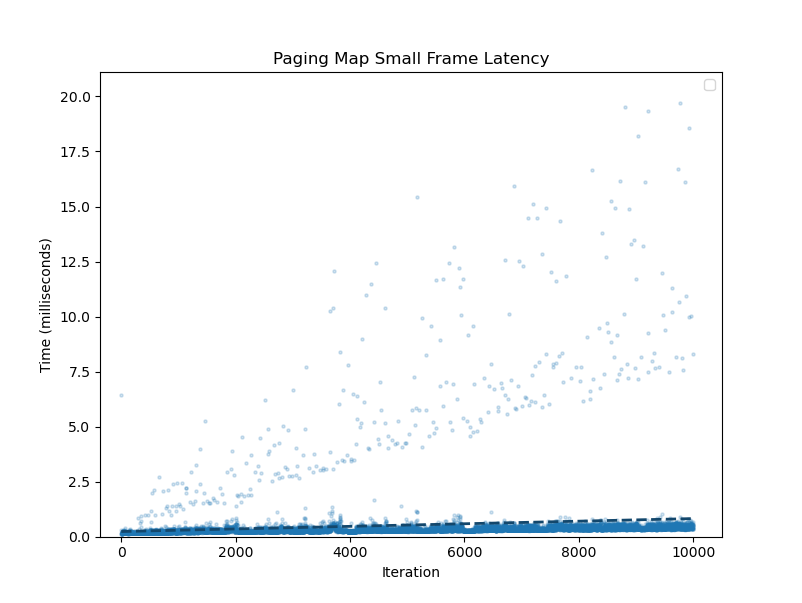
\includegraphics[width=0.58\columnwidth]{images/paging_map_small_frame_scatter.png}
        \caption{Mapping a series of 1-page frames.}
        \label{figure:paging_map_small_frame_scatter}
    \end{figure}
    \item \textbf{Figure \ref{figure:paging_map_large_frame_scatter}}: We evaluated the latency of mapping a series of large frames (100 pages each). There is a higher density in the second band compared to our small-frame-mapping test since a larger ratio of requests result in the creation and mapping of new VNodes. The per-iteration increase in latency is still small which may indicate that hash tables are effective for efficient VNode accesses.
    \begin{figure}[ht]
        \centering
        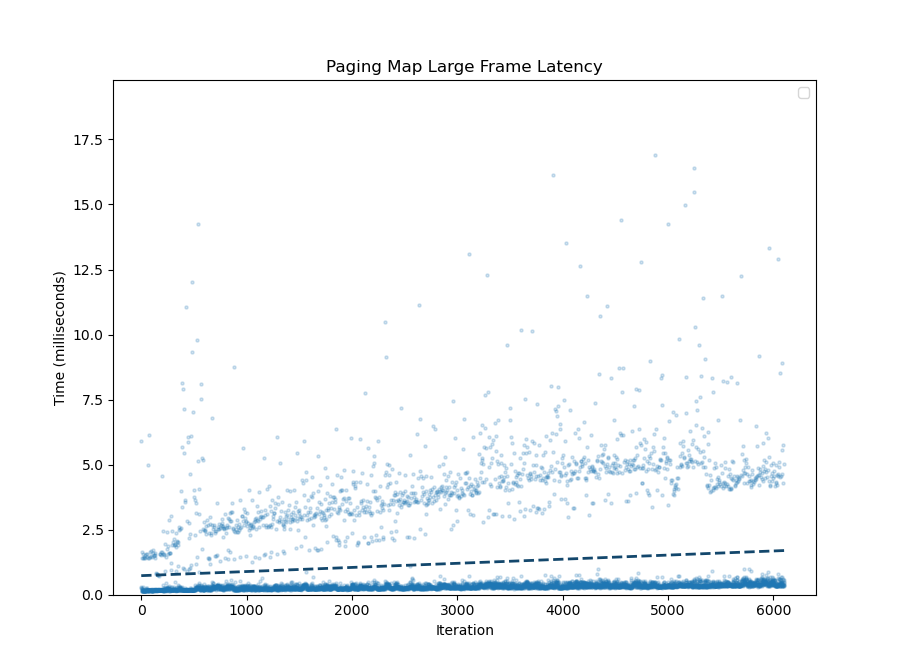
\includegraphics[width=0.58\columnwidth]{images/paging_map_large_frame_scatter.png}
        \caption{Mapping a series of 100-page frames.}
        \label{figure:paging_map_large_frame_scatter}
    \end{figure}
    \item \textbf{Figure \ref{figure:malloc_scatter}}: We evaluate our \texttt{malloc} implementation by allocating a large array and then causing page faults by accessing new pages on each iteration. The latency appears to grow linearly which falls in line with the linear growth of memory manager allocations and paging frame mappings. The latency surpasses 2ms after 5,000 page faults which is less than ideal and may require revisiting our generic allocator implementation should it become a bottleneck.
    \begin{figure}[ht]
        \centering
        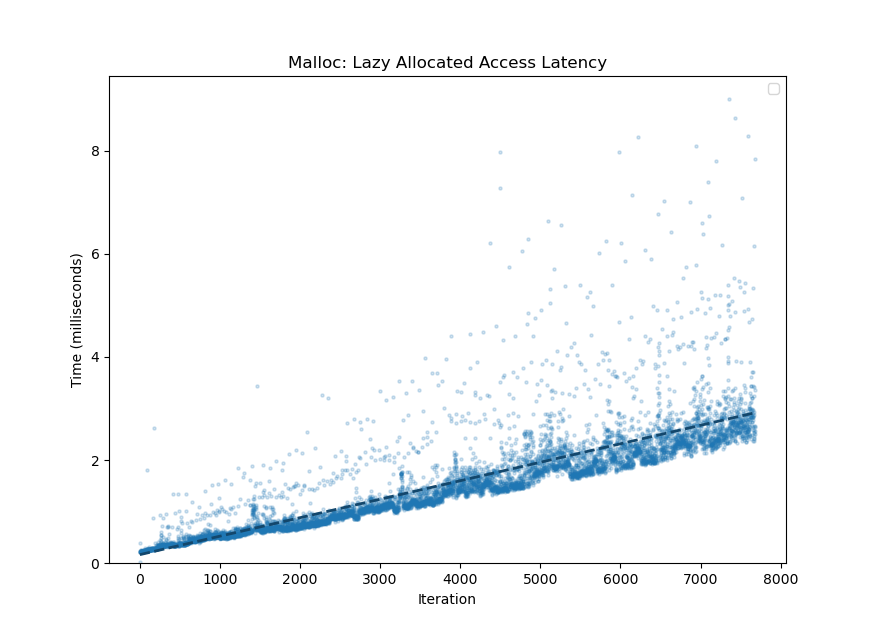
\includegraphics[width=0.58\columnwidth]{images/malloc_scatter.png}
        \caption{Page accesses in a lazy-allocated memory chunk.}
        \label{figure:malloc_scatter}
    \end{figure}
\end{itemize}

\newpage

\section{Spawning Processes}
We now have physical and virtual memory management systems running. Everything is in place to start spawning (and managing) processes, which is what we set out to do in this chapter. In Barrelfish, the way we go about this is by having another already existing process allocate space for the new process and map it according to the provided binary. This ``spawn" technique is to be contrasted with the Unix ``fork-and-exec" method wherein a ``parent" process duplicates itself and then the duplicated ``child" process replaces itself with a new binary. In terms of managing processes, we want to be able to map between unique, per-process IDs (PIDs) and metadata related to the associated process. This is a desirable feature because it allows us to do things like check what processes are running, suspend/resume processes, and more.
\\\\
Implementation steps for this Milestone were relatively linear since there were not too many design decisions to make, and the tasks were not as parallelizable compared to previous Milestones due to the bulk of work being in getting a new process to spawn. We therefore speak mostly about the sequence of steps required to spawn a new process in this chapter. Also note that, although it may seem as if concurrency (out-of-order execution steps in our system with no effect on outcome) is a problem to worry about in this Milestone, we are still only running our OS on a single core. The following implementation descriptions therefore do not account for this.

\subsection{Finding and Mapping the ELF Binary}
The first step to spawning a new process is to find the file that we want to execute (an ``ELF binary") and hand it to the new process (map it into its address space). Since Barrelfish conforms to the multiboot specification for its boot images and because no filesystem was yet available for this Milestone, the process binaries are stored in the operating system's boot image. In simpler terms, this just means that we put the processes that we want to spawn at well known locations (predefined physical memory frames) on startup. These frames include the binary's executable code as well as any default command line arguments to supply it with. The binary is then mapped into the parent process' virtual address space, as it must be able to access it in order to create the child process' mappings.

\subsubsection{Creating the CSpace}
Processes in Barrelfish expect certain capabilities to exist in well-known areas in its CSpace. This means that the next step is to construct the CSpace of the child process. This involves creating a new L1 CNode (the root) and a few required L2 CNodes (descendants of the root):
\begin{itemize}[itemsep=0pt]
    \item \textbf{Task CNode}: This contains process-specific capabilities such as ones for the dispatcher control block (containing information about the process), the frame containing process arguments, the ``early" memory used for initial memory allocations (allocating memory takes memory!), and more.
    \item \textbf{Page CNode}: This contains all of the page table capabilities of the process. Since page tables are themselves in memory, they also have associated capabilities.
    \item \textbf{Slot Alloc 0/1/2}: These contains space to store capabilities for the process' slot allocators.
\end{itemize}
Similarly to how the ELF image had to be mapped into the parent, any child capabilities that are to be invoked must also be copied into the parent's CSpace since the parent counts as a separate process from the child and thus cannot use its capabilities. Once these copies are no longer needed by the parent, they are deleted.

\subsection{Creating the VSpace}\label{m3-2}
Once the child's CSpace is set up we can set up its virtual address space (``VSpace" for short). This is necessary so that the child process has some initial memory to use, enabling it to allocate more memory for itself and subsequently manage it.
\\\\
As described in the previous section, one of the initial L2 CNodes required by the child process is the Page CNode which is where the root (L0) page table and all sub-page table (L1, L2, L3) capabilities are stored. Thus, we create the root page table, place it in the first slot of this CNode, and then allocate the remaining page tables by using a \texttt{single\_slot\_allocator} which is a slot allocator for a single L2 CNode. The rest of the VSpace setup is carried out analogously to how it was done in Milestone 2 for the initial \textit{init} process, with a difference being that any capability invocations involve copying the child capabilities into the parent's CSpace as mentioned earlier.

\subsection{Parsing the ELF binary}
Once the CSpace and VSpace of the child process is setup, the next step is to parse the executable information from the ELF binary and load it into the child's memory. Just like how the parent process copies the child's capabilities into its own CSpace in order to invoke them, the executable segments of the ELF binary must be mapped into the parent so as to further copy and modify them. Once this is done, the parent can then begin loading the segments into the child process' address space. The placement and alignment of these segments is given by additional metadata contained in the ELF. The actual loading step is carried out by the function \texttt{elf\_load} that is given to us; we simply had to implement \texttt{spawn\_elf\_allocator\_fn} which is responsible for mapping the executable segments to a given address.

\subsection{Setting up the Dispatcher}
We now need to setup the dispatcher's metadata. ``Dispatcher" is Barrelfish terminology for a process (or more technically, a ``schedulable unit"). This involves creating a capability to the dispatcher and a capability to its frame, both of which are stored in the child's CSpace (and again, copied into the parent's CSpace to invoke them). This frame stores information such as the physical core the dispatcher is to be run on, its PID, whether or not it is to be started in ``disabled" mode, etc. Dispatchers may also for some reason be stopped in lieu of another dispatcher at any time, so its associated frame must also store register state when context is switched in order for it to know where it last stopped when it starts again. Lastly, the dispatcher frame also needs to know the location of the ``global offset table" which stores all of the binary's global variables, else it would not know where they are located in memory.

\subsection{Setting up the Environment}
The final step before a process is ready to be spawned is to set up its environment. For a Barrelfish dispatcher, this includes the arguments to the binary, some initial RAM capabilities so that the process can bootstrap its own memory allocations, and any capabilities that need to be passed to the child. In terms of the arguments, this amounts to creating the frame, mapping it into both the parent and child process, and then copying the arguments into it. The RAM capabilities are then split from the parent's RAM capabilities (in our case, \textit{init}) and passed into the child's CSpace by way of the well-known \texttt{TASKCN\_SLOT\_EARLYMEM} slot in the Task CNode. Lastly, any capabilities to pass to the child are copied into the child's \texttt{ARGCN} L2 CNode. 

\subsection{Process Management}
We implemented a variety of process management functions which allow procedures to programmatically identify, pause, resume, or kill a process. Processes are identified uniquely by process ID, so we need a data structure to maintain a list of all process IDs and their respective states. Since we had already implemented a hash table for Milestone 2, it was easiest for us to repurpose it as a data structure associating process IDs with their state. Using this hash table, our process management library can efficiently look up state and other necessary metadata in order to perform operations on a process.

\subsection{Passing of Paging State to the Child Process}
Once a child process has successfully been spawned and before it can begin running any user-written code, it must perform some initialization steps so that it can access and use memory. One such step sets up the child's paging state, i.e. the means by which a process maps physical memory into its VSpace. Note however that as we described in \hyperref[m3-2]{Section 4.2}, on creation of the child's VSpace we must already have had to set up this paging state in the parent process in order to map the child's ELF segments into its VSpace. Due to this re-initialization the child does not know what has already been mapped by the parent and may try erroneously map a frame to an already-mapped memory region. In order to fix this, we want to pass this already-initialized paging state data to the child once it has successfully spawn, giving it knowledge on what already resides in its VSpace.

\subsubsection{Shared Frames Between the Parent and Child}
During the setup of the child's VSpace, the parent process creates a frame holding the child's paging state data. After initializing the child's paging state (still within the parent process), we then map this shared frame into the child process' VSpace and copy the paging state data into it. We must map this frame for the child rather than just giving the child a capability to the frame because it needs access to this data in order to perform any mappings. 
\\\\
In order for the child to find this data after it has spawned, the parent maps it to a well-known virtual address. During the child's initialization phase, the child checks if this well-known address does indeed hold valid paging state data and will make use of it instead of creating a fresh paging state for itself. Once and if the child has retrieved this paging state it no longer needs to keep the shared frame around. We copy the paging state data into its stack and unmap the frame from the child process.
\\\\
We employ a shared frame between the parent and child process for the purpose of passing paging state because at the point in Milestone 3 we don't yet have any other possible method of sharing data between processes (this changes in Milestone 4 where we develop a proper method of communication between processes). Even with an established communication protocol however, we still require the ability to self-page (available after paging state is initialized) in order to set up communication channels. A primitive and shared physical frame therefore seems to be the only way through which we can pass pre-initialized paging states from parent to child processes. 

\subsubsection{Ensuring Valid Virtual Addresses After Passing}
Simply copying data from a parent process into a frame that is then read in the child process does not work out as smoothly as we had initially hoped. The parent process' pointers reference addresses in a completely different address space from that of the child's so we must ensure that the passed paging state data will refer to valid addresses in the child's VSpace. We came up with two approaches to ensure this:
\begin{enumerate}
    \item Shared data structures and pointers between the parent and child should always refer to the same virtual address.
    \item If (1) cannot be enforced, the child's pointers must be updated to valid addresses once the process has started.
\end{enumerate}
An example of the first approach can be seen in the numerous data structures used to manage the VSpace as detailed in our \hyperref[M2]{Milestone 2}. These data structures are created for the child's paging state in the parent process during the spawning setup, so we map the frames holding these data structures and any of their accommodating buffers at the same addresses in both the parent and the child. When the child process tries to access these data structures during self-paging, its pointers will still reference mapped addresses in its VSpace.
\\\\
The second approach is necessary for data structures that use function pointers which are defined symbols in the parent's ELF image and thus are not valid in the child's VSpace. Once we are in the child process and have successfully retrieved the paging state data at the well-known address, we must update all function pointers within the paging state's data structures to refer to function addresses defined within the child's ELF image.
\\\\
There is one more step to ensure that all references in the passed paging state are valid within the child's VSpace. During creation of the child's VSpace in the parent process, we allocate a few starting page tables such that we can map in the child's ELF segments. The capabilities to these page tables all refer to a root L1 CNode existing at a CSpace address relative to the parent's CSpace. The kernel will not be able to resolve the page table's CSpace slot when we try to create a mapping, so we must now also iterate through any allocated page tables and update their associated capabilities to reference a root L1 CNode relative to the child's CSpace.

\subsubsection{Assumptions}
Using a shared frame between processes works without issue at this point of time in the Milestone where we only have one core and are running at most one thread at a time. In other words, this approach to sharing paging state data from the parent to the child is not thread-safe. In later milestones, many issues begin to arise when multiple procedures are spawning concurrently, causing the parent process to sometimes overwrite data in the shared frame before the child process has gotten the chance to read from it. It is then, that we introduce mutual exclusion to address this.

\newpage

\section{Message Passing}
As of Milestone 3, our operating system now has access to a fully-fledged memory management system and also supports the spawning and management of arbitrary processes. There still however remains the issue of how processes \textit{talk} to each other. Take for instance our process manager (which currently runs inside the \texttt{init} process). If some arbitrary process \textbf{A} wanted to wait on the execution state of another process \textbf{B}, it would need to query \texttt{init} on the state of \textbf{B} in order to do so. Ideally, we would also in the future like to separate services out from \texttt{init} such that the operating system's architecture resembles something more service-oriented. That is, we would have the physical memory manager, process manager, \texttt{init}, etc. all running as their own separate processes. How might they communicate with each other? In this Milestone, we implement remote procedure calls through LMP.

\subsection{Design Constraints}
At a high level, a remote procedure call (RPC) is just as the name suggests. It is a function that lives outside of the scope of the calling process (in our case, it lives inside another process on the machine). Obviously this requires some sort of communication; both processes need to agree on how the RPC call is invoked, what the parameters look like, what the possible return values look like, as well as how all of that data is organized when being sent through the underlying transport layer (in other words, they need to agree on protocol). In practice, this looks like:
\begin{itemize}[itemsep=0pt]
    \item The client invokes a local RPC stub, which: \begin{enumerate}[itemsep=0pt]
        \item Marshals any provided arguments into a buffer.
        \item Sends this buffer over the underlying communication medium.
    \end{enumerate}
    \item The server receives the buffer, and: \begin{enumerate}[itemsep=0pt]
        \item Parses out which procedure is to be called.
        \item Unmarshals any provided arguments.
        \item Calls the procedure with the provided arguments.
        \item Marshals any return values into a buffer.
        \item Sends this buffer back over the communication medium.
    \end{enumerate}
    \item The client receives the buffer, and: \begin{enumerate}[itemsep=0pt]
        \item Unmarshals the return values from the buffer.
        \item Returns these values back to client through the stub.
    \end{enumerate}
\end{itemize}
The RPC calls we set out to implement in this Milestone were those for memory management, process management, and terminal support. All calls were done using ``lightweight message passing" (LMP) for transport, which is a non-blocking, event-driven interface that allows us to send small payloads between processes on a single core. It can be thought of as loosely analagous to a transport layer protocol. Communication happens over a ``channel", which consists of two processes holding a capability to the other's endpoint. The big challenges for this Milestone were:
\begin{enumerate}[itemsep=0pt]
    \item How does a process find a server (e.g. whoever is handling memory requests) in the first place?
    \item Do we want all communication happening over one channel, or multiple? When should these channels open/close?
    \item Since LMP only provides us with raw payload exchanges, how do we pack our messages so that servers know what RPC is being invoked and what the arguments are? How do we pack our messages so that clients can retrieve return values and/or know the status of their calls? It would be preferable to build this in a way that supports any underlying transport layer (not just LMP).
    \item How do we send/receive messages that are larger than what LMP supports (in one send)?
\end{enumerate}
There are many degrees of freedom here. In contrast to past Milestones however, we were mostly concerned with designs that were simple, extensible, and isolated. Since Barrelfish supports other methods of communication (see Milestone 6), we wanted our messaging layer to not have to \textit{know} that it was using LMP. We also wanted it to be easy to do something like add new servers and RPC calls, since memory/process/terminal servers are certainly not the only things a complete OS may run.

\subsection{Binding}
If a process $A$ wants to send an RPC to process $B$, it uses an endpoint. Simply put, endpoints are capabilities to parts of a process' memory used for IPC. When $A$ sends a message to $B$, it sends it using its remote endpoint ($B$'s local endpoint). When $A$ wants to receive a message from $B$, it listens for it using its local endpoint ($B$'s remote endpoint). This is fine, however we still need to get $A$ and $B$ to give each other their endpoints in the first place, otherwise they won't know where to send messages. In other words, we need them to ``bind" to each other. Since we don't have a nameserver running (yet), this Milestone requires some amount of hardcoding in order to give processes knowledge of the available servers.
\\\\
We decided to put all functionality for this Milestone into \texttt{init}, so in effect we have a single process serving all RPC requests (explanation for this choice is explained later). The way processes bind to \texttt{init}, then, is as follows:
\begin{enumerate}[itemsep=0pt]
    \item When \texttt{init} spawns a child process, it puts its self-endpoint into a well-known place in the child's CSpace.
    \item When the child process starts, it creates a ``self-endpoint" and stores it in a well-known place in its CSpace. The endpoint refers to itself. Since it has \texttt{init}'s endpoint (the remote)  from the spawning process and its self-endpoint (the local), it creates a channel between the two.
    \item The child process sends its self-endpoint to \texttt{init} using the channel, allowing \texttt{init} to build its side of the channel.
\end{enumerate}

\subsection{Exchanging Messages}
\subsubsection{Messaging Layer}
Since LMP only gives us the ability to send raw buffers of data, we need syntax and semantics for our messages in order to know what RPCs are being invoked, as well as the arguments being provided. We also need this in order to retrieve return values, and to know \textit{if} and \textit{when} our requests have been served. LMP supports a maximum payload size of 8 words and 1 capability reference. Our messages are packed as follows:
\begin{itemize}[itemsep=0pt]
    \item 0: Message Type - specifies what kind of message is being sent. This encapsulates both request and response messages.
    \item 1: Thread ID - specifies the ID of the calling thread. This is necessary since multiple messages can be in-flight at once, so we need a way to identify \textit{who} has made the request to return the response to.
    \item 2: Result - specifies the error/OK response resultant after serving a request. This field is only interesting for callers when they receive a response.
    \item 3-7: Arguments - contains parameters if the message is a request, or return values if the message is a response.
    \item Capability - sometimes we need to send or receive a capability (for example when requesting memory, or during binding). If not, then this is set to \texttt{NULL}.
\end{itemize}

\subsubsection{Thread Multiplexing}
LMP is non-blocking and event-driven. This means that when we call an LMP function we need to provide it with a callback, which will execute at an indiscriminate time in the future when the call is processed. Programmatically, the function itself returns immediately. Assuming the call is made on thread $A$, we handle cases where we need to block on a response as follows:
\begin{enumerate}[itemsep=0pt]
    \item Thread $A$ creates a ``message loop", thread $B$, which will continue to receive messages (and execute their callbacks) on the channel while $A$ waits for the response its interested in.
    \item Thread $A$ sends its request and begins blocking on a semaphore. We use a semaphore because, under low system load, the response to our request may be received before we even need to start blocking the thread.
    \item When the response comes, thread $B$ executes the associated callback, which posts to $A$'s semaphore and thus unblocks it.
    \item Thread $A$ reads the response and continues as usual.
\end{enumerate}
Note the necessity of the message loop. Since the caller needs to block when waiting for a response, something still needs to be running in order to unblock it when the response comes. The message loop waits on a ``waitset", which is an event queue, and dispatches events as they arrive. Dispatching an event triggers a closure registered with the waitset, and it is in this closure that we decide which thread to unblock based on the thread ID in the message.
%The same functionality can be achieved using a ``waitset", which we explore in depth during Milestone 6. The library for these was pre-provided and would have arguably been a cleaner way to handle message passing, but due to time constraints we were not able to figure out how they worked. We instead opted for a more familiar route (and ironically ended up with a partial re-implementation of waitsets).

\subsection{Servers}
All RPCs are handled through a connection to \texttt{init}. In effect, it serves as the memory, process, and terminal server all at once. Basic coding practices say that a separation of concerns would have been better here, however we once again made this decision due to time constraints. The issue is consequently handled in Milestone 7 with the introduction of a nameserver. If we had done it in this Milestone however, the binding process would have been replicated for each server by defining well-known capability slots and handing them off to any spawned processes. Each server would be connected separately to bound processes, and only know about a partial set of the RPCs we implemented (everything would still go through the messaging layer and LMP).
\\\\
Implementation here was relatively straightforward since we already had all of the pieces for memory management, process management, and terminal reads/writes. We just had to integrate it with our communication subsystem.

\subsubsection{Memory Server}
The memory server (\texttt{init}, in reality) allows clients to request RAM capabilities. This is done using LMP's support for passing capabilities; when the client requests $X$ bytes of RAM, the server's memory manager will allocate at least that amount and then pass its associated capability reference in the response message. This allows the memory manager to allocate RAM and hand it out to processes while maintaining a unified view of memory usage on the system (which is required, otherwise multiple processes may erroneously make accesses to each other's memory).

\subsubsection{Process Server}
The process server handles everything to do with process management. Just like the memory server, this gives our system a single point of control for process management and thus a full view of all processes on the OS, their states, identifiers, etc. The process server supports RPCs for all functionality provided in Milestone 3 including spawning, killing, status fetching, pausing/resuming, etc. 

\subsubsection{Terminal Server}
The terminal server gives us a way to send and read characters from the terminal through RPCs. This can be useful, for example, when writing drivers for something like a UART. Standard library functions can be overridden to use our read/write RPCs (in fact, we do this) for terminal functionality.

\subsection{Large Messages}
Sometimes we may want to send a message that is larger than the size supported by LMP. For example, calls to the process server asking for a list of PIDs may be arbitrarily long. In this case, we use LMP's capability passing feature. To do this we request a frame from the memory server, fill it with the necessary arguments/return values, and then send it over the channel.
\\\\
While this technique works and may even seem like a clever use of capability passing, we realized in hindsight that it is not \textit{extensible}. In Milestone 6 we add support for a different transport layer called ``UMP", which cannot pass capabilities safely. A different and arguably better approach would have been to send a series of messages, each containing chunks of the data. A ``header" message would be sent first indicating that the data doesn't fit, followed by the data and a ``footer" (indicating the end).
\\\\
This served as an example of where doing things the ``easier" way actually turned out to cause more headaches. While on first glance passing a frame seemed like the simplest way to do things, our lack of foresight came back to bite us since we ended up having to redo our implementation in order to support other transport layers.

\newpage

\section{Multicore Support}
Up until now we have been implementing our operating system on the assumption that it runs on a single core. With the introduction of message passing in the last Milestone, we are at the point where we can start harnessing the full power of the underlying computer's CPU by using all of its available cores. In this Milestone we implement multicore system support for our OS and begin thinking about cross-core communication.
\\\\
Barrelfish is a \textit{multikernel}. Instead of running all operating system services in a single address space (a ``monolithic" kernel), it treats multicore machines as a distributed system. That is, each core on the system runs its own kernel in a separate address spaces. Instead of assuming shared memory for inter-process communication (IPC), we rely primarily on message-passing (similar to LMP) for synchronization and distribution of workloads. In this case, system invariants are enforced not through locks, but through distributed algorithms.
\\\\
Our goals in this Milestone didn't require too much thought about design. We were interested mainly in successfully booting a second core, giving it a subset of the physical address space, and getting some sort of primitive communication going between it and the first core. We provide a walkthrough of how each of these things were achieved.

\subsection{Booting a New Core}
The first thing to do is allocate memory for the new core. We use our memory manager to allocate RAM for the various bits and pieces necessary, and then store their base addresses and sizes in the ``Coredata" structure. Coredata stores boot paramaters for the new core such as its ID, how much memory it has, and as we just mentioned, where to find the memory it needs for initial execution. Note that our bootdriver and CPU driver use the kernel page table, which implements a 1-to-1 mapping between physical and virtual address space (in other words, we're using physical addresses). Also note that we must \textit{relocate} the bootdriver and CPU driver since they are linked to run at a specified address, but in reality run at another. The result is that global variables now have differing addresses and thus need to be relocated. The new core needs the following:
\begin{itemize}[itemsep=0pt]
    \item The ``kernel conrol block" (KCB), which stores the state of the kernel, requires memory. We need to provide an empty state for the new core to start with, after which it will handle this on its own. We allocate RAM, retype the RAM to a KCB capability, and then store its physical address in the Coredata.
    \item \texttt{init}, since this will be the first process to run on the new core once it boots. We load the binary and store its size/physical address in the Coredata.
    \item The bootdriver/CPU driver, which start up the core when we tell it to begin (the CPU driver keeps running after boot as well). The CPU driver is allocated, loaded, and relocated, with its entrypoint being stored in the Coredata. The bootdriver is also allocated, loaded, and relocated, however it is instead handed back to the caller since it is run using multiboot, which are just binary images built into the OS to allow us to run applications without a full-fledged filesystem.
    \item At least 16 pages of stack memory for the CPU driver, necessary for its execution. We allocate this and store the size/physical address in the Coredata.
    \item A small amount (roughly 5MB) of memory to get the core running. Remember that it cannot manage its own memory during startup, since \texttt{init} has not even begun running. The size and address of the memory is stored in the Coredata.
    \item A URPC frame, necessary for cross-core communication. We explain this in-depth at a later time. Its size and address are stored in the Coredata.
    \item The location of the multiboot strings. We need this particularly to spawn processes from the multiboot images. Its address is stored in the Coredata
    \item The physical address to memory holding Boot information structure, which has the physical addresses of starting RAM regions for \texttt{init} to add to its memory manager. This structure also includes addresses to the ELF images from multiboot modules, which is necessary for spawning processes without a functioning filesystem.
\end{itemize}
Once we have all the information necessary for the new core's Coredata, we allocate it, fill it in, and get its physical address, which will subsequently be handed off to \texttt{init}. Before the call to \texttt{init} however, we need to ensure that the data we've written is visible to the core, since its MMU will not yet be on. This requires a data-memory barrier (guaranteeing that all loads and stores up to this point in execution have completed) and a cache invalidation/clean (to ensure that all information is fresh and actually in memory). Finally, we may invoke the monitor (\texttt{init}) to spawn our new core.

\subsubsection{Memory Allocation on New Cores}
Remember that in a multikernel, each core is running its own instance of the kernel with its own part of memory. We now have the core booting part done, but we still need to figure out how to split and hand off memory to each core. We implemented a rather simple technique to achieve this, just to start off. The approach is basically to manually split memory for each core; since we were only concerned with running two cores to start, the first core checks if it is, in fact, the first core. If this is the case, its (the first core's) memory manager takes half of the available physical memory and marks it as in use. On boot, the second core confirms that it is not the first core, and then ``forges" capabilities for the available remaining, unmarked RAM (the other half). That RAM is then handed to its (the second core's) memory manager. The operation of forging RAM invokes the kernel capability to create a new capability for a given region of physical memory. This ``forging" must be done, since each core runs its own CPU driver and monitor---there is currently no concept of passing capabilities between cores (this is updated in the Capabilities portion of Milestone 7).
\\\\
Note that a slightly more clever scheme could be used here to divide the address space based on an arbitrary amount supported cores, but this would be trivial (in theory...) and we were only concerned with the two-core case to begin. Also note that we \textit{must} start off new cores with some amount of physical memory since they need to actually be able to run a few operations in \texttt{init} to set up communication channels to request more memory dynamically. After this happens however, processes on cores may begin to exchange RAM through IPC.

\subsubsection{Spawning Processes on New Cores}
In order to spawn processes on our new core, it needs to have access to the multiboot modules, which contain address to their ELF images in memory. This is quite straightforward since we have all of the pieces necessary to do this already. The ``boot info" structure handed to the new core contains an array of memory regions; some may be marked as multiboot modules, so we do a search for them, For any found modules, we invoke the kernel capability to forge a frame capability pointing at the module, and we're ready to go. Since the new core has the module in memory, its location, and a capability for it, we can now spawn the associated process just as was done in Milestone 3.

\subsection{Cross-Core Communication}
This part of the Milestone serves as an introduction to communicating between cores; Milestone 6 will explore this in depth. Remember yet again that we're building a multikernel, which means that each core works as a node in a network running its own instance of the kernel. Cross-core communication therefore is vital. Before implementing a full cross-core IPC system in Milestone 6, we start by implementing a simple shared-memory communication channel between our two cores.
\\\\
When booting new cores, a ``user-level RPC" (URPC) frame gets allocated. The URPC frame is a piece of shared memory between cores that we can use to communicate over, using ``UMP" (user-level message passing). After the second core boots, a UMP frame is mapped, initialized, and its channels are opened. In order to actually communicate over the frame, we use a ring buffer. Sending messages involves writing our data to the buffer and then setting a ``control word" at the end when the data is ready to be received. Receiving messages involves polling on that control word and then reading the associated data when it is ready. When a message is confirmed as received, both sides of the channel can advance their pointers in the ring buffer. Note that in contrast to LMP, UMP supports full-duplex connections using \textit{two} channels; one for sending, and one for receiving.
\\\\
During Milestone 5, we did not start with a rudimentary communication protocol, but started to implement UMP in its entirety as we felt that it would be more efficient to do so. Thus, we reserve the details for this communication protocol, as it is the primary topic of the following section. 

\newpage

\section{Cross-Core Message Passing}
Our IPC implementation from Milestone 4 only handles processes that are running on the same core. With the introduction of multicore support in Milestone 5, we now must handle the case where processes are talking to each other \textit{across cores}. Remember that Barrelfish is built as a distributed operating system; this issue is paramount to reaching a fully-fledged system and we tackle it in this Milestone.

\subsection{Design Constraints}
In Milestone 4 we used LMP. Our goal now is to use ``User-Level Message Passing" (UMP) to achieve cross-core communication. UMP uses shared memory (URPC frames, one per connection) to pass messages, and supports full-duplex communication through 2 unidirectional channels (one for sending and one for receiving). For performance purposes, it avoids kernel context switches (hence ``user-level"), and communicates purely through cache lines when possible. This is possible under the assumption that our processor employs the ``MOESI" cache-coherence protocol, where reading dirty cache-lines can bypass a write-back to memory by obtaining the cache line directly from the core that ``owns" the cache-line \cite{armman}.
\\\\
Since we already implemented a messaging layer previously, our main goal in this Milestone was to implement UMP. Our design choices here mainly lent themselves to speed because IPC is crucial to many multikernel operations, and we wanted to use UMP over LMP whenever possible. As always there was a time constraint, so we also opted for simple design choices in place of more complex ones. Finally, we needed to keep in mind that both UMP and LMP are transparent to userspace processes, so it is our decision on which protocol various processes will use to communicate. Going in, the main challenges we identified were:
\begin{itemize}[itemsep=0pt]
    \item How does one bind to a service running on another core?
    \item How should the URPC frame be arranged for message passing? Where does a message start, and how long will it be?
    \item If a message is ready to be sent/received, how does the other side know? We need to guarantee that what we're reading is actually a new message, otherwise we might end up re-reading old ones. Likewise, we might end up overwriting unread messages on the sending side.
    \item Messages could possibly be larger than what UMP supports in a single send, or larger than the entire URPC frame itself. What do we do in this case? This was done in Milestone 4 with our messaging layer, but we realized that our implementation was not ambivalent to the underlying transport layer (more on this later).
    \item We currently have one instance of each resource server running (e.g. each core has its own process manager, memory manager, and serial server). How should we coordinate and synchronize them?
\end{itemize}

\subsection{Binding}
Assume that a process \textbf{A} on core \textbf{1} wants to talk to a service \textbf{B} on core \textbf{0}. Recall that in Milestone 5, \texttt{init} on core 1 is given the physical address of a frame by \texttt{init} on core 0 to set up as the URPC frame, allowing them to communicate. This only works because \texttt{init} is a privileged process that can generate new capabilities from a given physical address (``forging"). This is where the concept of the \textit{monitor} comes in. Up until this point, we have been referring to \texttt{init} as ``just another process", with its only defining part being that it is the first process to run. In this Milestone and onwards however, we will refer to it as the ``monitor" and give it its first special job: to help processes bind to each other across cores. It is able to perform this job because of its ability to forge capabilities.
\\\\
For simplicity we have been housing all resource servers within the monitor up to this point, with the plan to separate them later in Milestone 7 when the nameserver is built. Thus, when we refer to a resource server in this section, we really mean the monitor. Suppose there is a child process, \textbf{A}, on core \textbf{1}, that wishes to communicate with a resource server on core \textbf{0}. The procedure for enabling communication between child processes and a resource server is as follows (Figure \ref{figure:m6-bind}):
\begin{enumerate}[itemsep=0pt]
    \item The child process \textbf{A} sends a frame capability (the frame in which UMP communication will occur) over LMP to its monitor (on core \textbf{1}).
    \item Core \textbf{1}'s monitor sends the \textit{physical address} of the frame to core \textbf{0}'s monitor via their UMP channel. The physical address is necessary because UMP currently cannot safely send capabilities (this changes in Milestone 7).
    \item Core \textbf{0}'s monitor forges a capability to the client frame and initializes an RPC channel to process \textbf{A}. 
    \item The client frame is split in half. From the server's point of view, one side is for sending messages, and the other is for receiving them. To the client, this view is flipped; the server's sending side is the client's receiving side, and the server's receiving side is the client's sending side. This is explained further in the following section.
\end{enumerate} 
Note that this binding procedure generalizes; one way to achieve communication between two processes across cores would be to have their respective monitors act as middle-men.
\begin{figure}[ht]
    \centering
    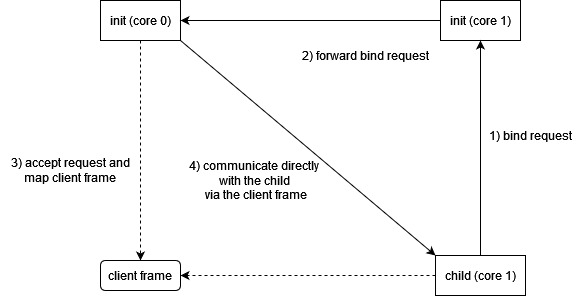
\includegraphics[width=0.8\columnwidth]{images/m6-bind.jpg}
    \caption{The sequence of events that occur during a binding request}
    \label{figure:m6-bind}
\end{figure}

\subsection{Transporting Message}
In Milestone 4 we built a generic transport interface to abstract RPC logic out from a specific transport protocol (Figure \ref{figure:m6-rpc-layout}). So, to add UMP support, we simply had to implement the generic functions for this interface without altering the RPC library functions.
\begin{figure}[ht]
    \centering
    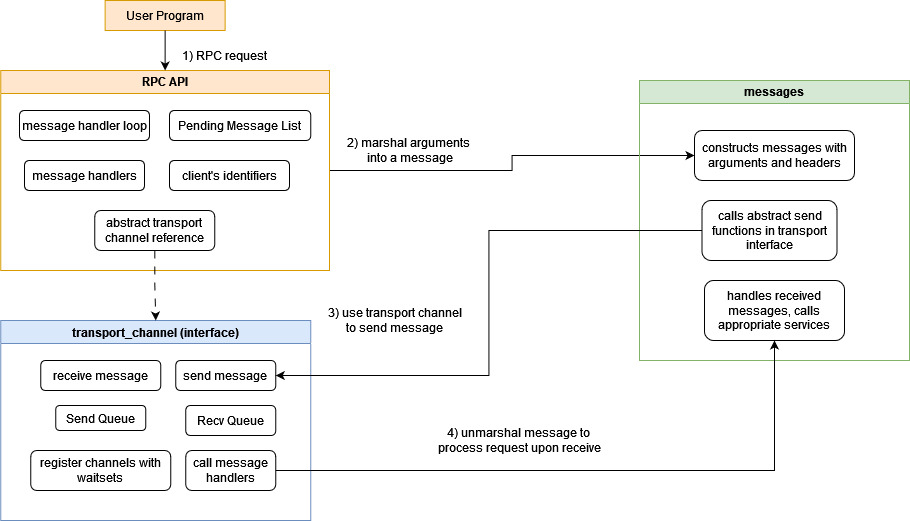
\includegraphics[width=\columnwidth]{images/m6-rpc-layout.jpg}
    \caption{The various layers involved in servicing an RPC.}
    \label{figure:m6-rpc-layout}
\end{figure}

\subsubsection{Ring Buffers}
We use a \textit{ring buffer} for UMP connections, which can be thought of as a queue that wraps back around to its start when its maximum size is reached. More specifically, we use two shared ring buffers: one for sending, and one for receiving. Since the buffers are shared between both sides of the connection, the sending buffer for one side will be the receiving buffer for the other and vice versa. Before getting any deeper, there is a bit of jargon to understand here:
\begin{itemize}[itemsep=0pt]
    \item \textbf{Slot}: A placeholder for a message in a ring buffer. This may contain the message, as well as other metadata necessary for proper handling of the message. From the perspective of the reader/writer this is atomic, just as a slot in an array is.
    \item \textbf{Waitset}: Acts as the connective tissue between threads and channels. For example, if we want to know when something is ready to be received on the channel, we use a waitset to poll for a \texttt{UMP\_IN} event, which tells us that something has been put into the receive buffer.
    \item \textbf{Control Word}: A reserved byte which each slot in a ring buffer contains. A \texttt{UMP\_IN} event only tells us that something has been written, but not if the message being written is finished, so we use the control word to do so. The control word is crucial in the synchronization of message content between the two cores, which is detailed in a later section.
\end{itemize}
On the receiving side, we use a \textit{waitset} to poll a \textit{control word} in the next \textit{receive slot}. That is, we hold a pointer into the next slot a message will be written into. Every time something is written, we check if the associated control word is set. If it is, we know that the message is ready and that we can begin to read and process it. On the sending side, we have to check if the buffer is full. If it isn't we can simply write the message (and set the control word when we're done), but if it is we use a waitset to poll until the receiver acknowledges a message.

\subsubsection{Memory Barriers}
Our system assumes an ARM processor, so we must take into account its ``weak memory consistency model``. The chip does not guarantee that memory stores/loads will occur in the order they are written by the program. This is particularly important for UMP since we use a control word between UMP clients and servers to signal whether messages are ready to be received. There is no guarantee that the sending core actually sets the control word \textit{after} it writes the message data, and similarly there is no guarantee that the client correctly checks the control word \textit{before} reading the message data. To solve this we employ the use of memory barriers, which ensure that load and stores occur in their intended order, while polling the UMP channel and receiving messages.

\subsubsection{ACKs}
How does the receiver acknowledge a message? In other words, how do we know what the receiver has and hasn't read from the ring buffer? This is necessary else we may end up overwriting unread messages, or re-reading messages that have already been read. The first idea we had was to have the receiver send an ACK over its sending buffer, signalling that a slot has been read in its receiving buffer, thus allowing the sender to reuse that slot. However, an ACK is also like any other UMP message---how do we know that an ACK has indeed been received? We can't send an ACK for a received ACK, as this clearly ends with an infinite loop. 
\\\\
One might reason that we can simply assume the ACK has been received (thus freeing that slot to be reused), however this is an unsafe assumption to make. In the case where the sender has not actually gotten around to processing the ACK and the receiver sends a bunch more messages to the point where the buffer does a full loop back around to the ACK, it will be overwritten and lost before being read.
\\\\
We figured that this problem may be solvable with extra checks and metadata, but we ended up opting for a more efficient (and arguably simpler) approach. Now, we reserve a slot in the ring buffer for ACKs (the ``ACK slot"), storing the index of the next unread slot. When the receiver reads a message from its receiving buffer, it increments the ACK slot index which points at the next unread slot. Before the sender puts a message in this buffer, it reads the ACK slot to check that the slot it is writing into doesn't contain an unread message. In order to handle cases where ACKs in the buffer have looped back around and thus overlap with the index, we use an additional piece of information in the ACK slot called the ``iteration number". This solution is a bit nicer than the previous because we always use at most 1 extra slot, no matter how many messages are sent. With the previous implementation, we required 2 slots for every 1 message sent (1 for the message, 1 more for the ACK).

\subsubsection{Large Messages}
In Milestone 4, when a message was larger than what a single send could handle, we would fill a frame with the excess data (arguments/return values) and then pass the frame's capability to the receiver. This turned out to be a major oversight on our part because UMP cannot arbitrarily pass frame capabilities in a safe manner (although Milestone 7 improves this). To do so with the current state of our system would require un-tracked forgings of capabilities on the fly, which can cause memory-consistency issues.
\\\\
In order to handle large messages (in a way that is ambivalent to the transport layer), we now have the sender split the data and send it as a series of smaller messages that each fit in a slot. The receiver accumulates the data in a buffer and forwards it to the appropriate message handler once the full message is received. Note that the message data chunks do not specify ordering because it is not necessary; this is the case because each RPC channel has its own individual waitset, which we explain next.

\subsubsection{Waitsets}
We previously used a single waitset for all RPC channels (specifically, the default waitset configured for a domain). This worked fine in Milestone 4, but it introduced a glaring problem with our system that surfaced with the introduction of UMP.
\\\\
With a singular waitset, all associated threads waiting on it will be woken up when \textit{any} channel picks up an event. If we have multiple RPC calls in flight on both LMP and UMP channels, threads that are meant to only service UMP requests will become triggered by an LMP request sent on the same waitset. This is particularly bad when we require sequences of an LMP call followed by a UMP call to service a request (e.g. during client-server binding), as the UMP handling thread will become blocked by accidentally trying to service the LMP request. Even if we somehow prevent this LMP-UMP problem, the wrong thread may continually pick up an event and then put it back on the waitset, resulting in randomly long processing times for RPCs.
\\\\
With our new message splitting scheme this becomes worse. Since multiple message handling threads might get events for the same channel, ordering and synchronization of large messages becomes an issue in the case that different threads pick up different parts of a large message. The obvious fix for us here was to refactor such that we register one waitset per RPC channel. This means that now, each thread waits on its own isolated waitset. Thus, large messages between two processes can only ever be handled by the thread it is intended for, ensuring that it will be received in order.

\subsection{Servers}
Previously, we had a single instance of each service running because we only had a single core to run them on. With the introduction of multiple cores, information required by a service may exist outside of its scope and so we must make some changes to the existing infrastructure. There are now three questions we must address with regards to our servers:
\begin{enumerate}
    \item Where will this server run? In its own process or within the monitor?
    \item Will we host this server on a single core, or will it be duplicated across cores?
    \item How will arbitrary processes communicate with this server; with LMP, or with UMP?
\end{enumerate}

\subsubsection{Memory Management}
Our memory management server starts off as distributed, but eventually devolves into a singular server. When core \textbf{1} boots up, it's given a portion of core \textbf{0}'s starting RAM capabilities. In the early stage of the system, core \textbf{1} may use this portion of RAM to service any requests, and thus the memory servers are distributed in that processes on either core will only request RAM from the memory manager on its local core. However, when core \textbf{1} inevitably runs out of this early memory, it will then begin to service any RAM requests by forwarding it via UMP to core \textbf{0}, thus the memory server becomes a single entity.
\\\\
We have also left the memory management server insidethe monitor since it is convenient for cross-core RAM requests. Core \textbf{1} must forge a capability upon receiving RAM from core \textbf{0}, and this can only be done within a privileged process, such as the monitor. As such, processes can only communicate with the memory server through LMP, as it requires involvement of their core's monitor. 
\\\\
We decided to only allow core \textbf{1} to request memory from core \textbf{0}. So, if a process on core \textbf{1} frees memory that it has used, core \textbf{0} cannot request that RAM back from core \textbf{1}. This is addressed later in Milestone 7.

\subsubsection{Serial I/O}
Our serial driver service currently does not need to manage any state. It simply prints output and retrieves user input. For now, it is compact enough to leave inside the monitor, but may be moved out once the shell is implemented in Milestone 7. Furthermore, there is no reason to centralize this server due to its lack of functionality (currently). Thus, we run a serial server on both cores. To make communication with this server faster, processes \textit{always} use UMP to contact it.

\subsubsection{Process Management}
We left the process management server inside of the monitor with the intent of waiting for the nameserver to be set up (Milestone 7) so that we could move it into its own process. The process management server must now be distributed in some sense, because processes may run on different cores. We identified two options:
\begin{itemize}[itemsep=0pt]
    \item \textbf{Singular Server}: This involves running a single instance of the process server. Information is centralized and thus cross-core communication is not necessary when serving requests; when RPCs are made to the server, the response is quick (relative to the second approach). One disadvantage however is that other cores need to communicate to the process server whenever one of their processes' states updates. This results in higher latencies across the board for process operations such as spawning, resuming, etc. since a message must be passed to the server in each case.
    \item \textbf{Decentralized Server}: Here, each core has a local process management instance that acts as a node in a network. This has the advantage of simpler bookkeeping, since each node simply has to store the state of processes local to its core (which is what we were doing before). The disadvantage is longer latencies when serving requests; if for example a request comes in to retrieve the list of processes running on the system, the local server handling the request must send a UMP call to all other nodes and then aggregate their data. Requests such as waiting on a process running on another core also require communication between nodes, since the local server only stores information about its own processes. In the end, we decided to go with the latter option. We already had an implementation with servers running on each core, so we simply had to tweak RPCs that now required communication.
\end{itemize}
There is one remaining question left, which is how a process may contact the two process management servers. This is not as simple as with the previous two servers, as we may want to obtain information about a process that is not running on our local core. In this case, it would make the most sense to send a UMP request to the other core's process manager to retrieve that information. Within the RPC interface, the process channel must be fixed to one type of protocol; the user does not care whether LMP or UMP is used when it tries to retrieve a reference to the channel to the process server. If we fix this channel to use UMP, what happens when a child process wants to obtain the status information of a process on its local core? We would have to send a UMP request to the other core's process server, which then sends a UMP request back to our current core's server, which would then send a UMP response back to the other core, and finally send a UMP request back to us, the requesting process (Figure \ref{figure:m6-ump-proc}.
\begin{figure}[ht]
    \centering
    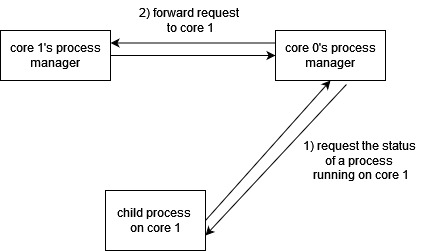
\includegraphics[width=0.8\columnwidth]{images/m6-ump-proc.jpg}
    \caption{The UMP calls that need to be made if the process server could only be contacted via UMP.}
    \label{figure:m6-ump-proc}
\end{figure}
\\\\
Although this seems strange and very roundabout, we hypothesize that despite the overhead of making more RPC calls (via UMP), it would still be faster to do this than to contact the process server through LMP. Our justification for this decision lies in the next section where we look at performance measurements. 

\subsection{Performance Measurements}
Our first question (and probably yours too) was ``is our UMP implementation actually faster than LMP"? To test this, we had a child process send a string of increasing length (which will require increasing numbers of messages, due to our long-message implementation) to \texttt{init} on its local core via LMP. We then compared the latency of these RPC calls with sending the strings to the other core's \texttt{init} via UMP. The results are observed in Figure \ref{figure:send-string-no-kernel}.
\begin{figure}[ht]
    \centering
    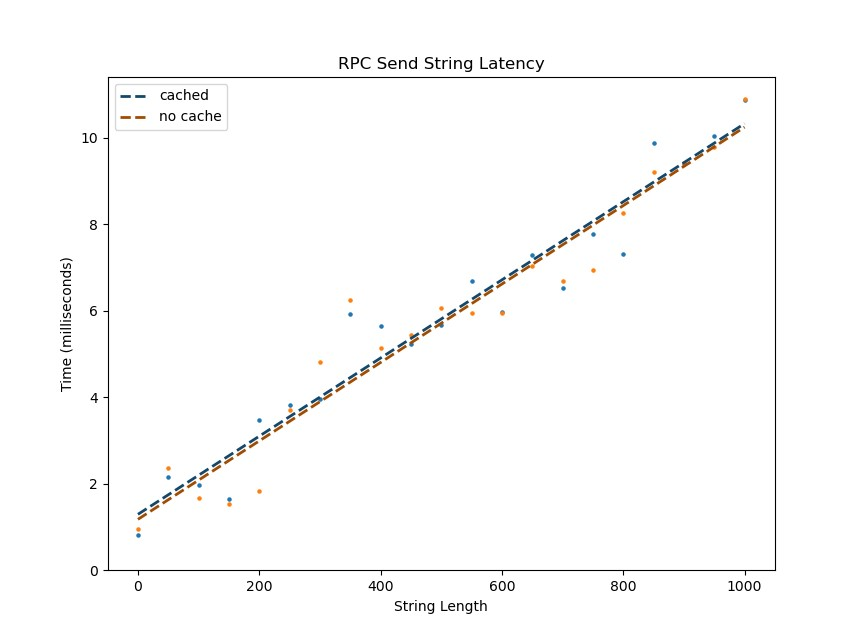
\includegraphics[width=0.8\columnwidth]{images/send-string-no-kernel.png}
    \caption{Sending a string via UMP vs LMP while under no kernel load.}
    \label{figure:send-string-no-kernel}
\end{figure}
\\\\
These are very alarming results. Our UMP implementation does not seem to be much faster than LMP. In fact, LMP also seems quite fast, as both  protocols service the request within approximately 10 milliseconds. We discussed various reasons for observing these results such as whether or not we had implemented UMP properly to exploit the ``MOESI" protocol (which allows us to bypass memory write-backs). 
\\\\
Discussions centered around our code did not lead to anything conclusive until we realized a key piece of information: this test ran on our system in isolation. The kernel was free to deliver and receive LMP messages, as nothing else was causing contention in access to the kernel. Furthermore, UMP also has the overhead of constantly needing to poll its channel for new messages, which would not make it faster in these conditions. We re-ran our tests, now with a simultaneously running thread that constantly used a capability operation requiring kernel involvement. The results are shown in Figure \ref{figure:send-string-kernel}.
\begin{figure}[ht]
    \centering
    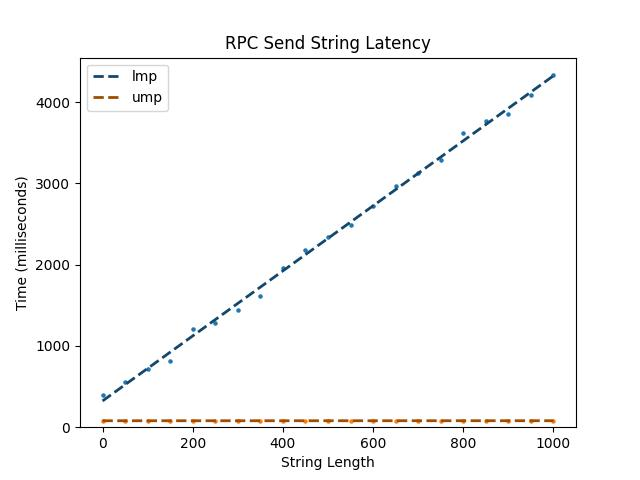
\includegraphics[width=0.8\columnwidth]{images/send-string-kernel.jpg}
    \caption{Sending a string via UMP vs LMP while under high kernel load.}
    \label{figure:send-string-kernel}
\end{figure}
\\\\
These results are much more in line with our expectations of UMP. Using these results, we now tested our hypothesis from the previous section about how processes should communicate with the process management server. Figure \ref{figure:proc-kernel} shows the latency of a process on core \textbf{1} requesting the status of a process running on its local core via LMP compared with UMP. This test was also run with a simulated kernel load.
\begin{figure}[ht]
    \centering
    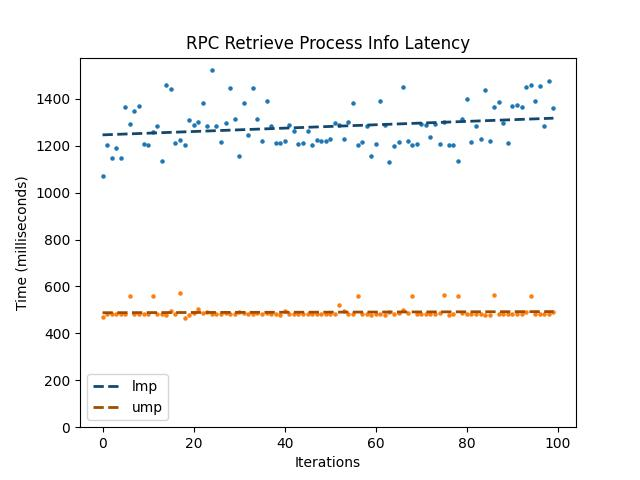
\includegraphics[width=0.8\columnwidth]{images/proc-kernel.jpg}
    \caption{Requesting the status of a process running on the same core via LMP vs UMP, under kernel load.}
    \label{figure:proc-kernel}
\end{figure}
\\\\
UMP is still much faster than LMP under kernel load despite requiring more message passing. We then made our decision to use UMP for contacting process servers based on these observations.
\clearpage

\newpage

\section{Networking}
For the final Milestone, each group member was required to individually implement different Barrelfish subsystems and then jointly integrate them at the end. This chapter delves into \textit{networking} and was completed by \textbf{Adrian}.
\\\\
Due to time constraints I was not able to get this milestone done, so the majority of this chapter is written from a ``what if" perspective. All design here is theoretical and may gloss over some finer details that only would have been revealed during the implementation process.

\subsection{Introduction}
A modern OS is not very useful without some way to communicate with the outside world. In order to achieve this, they all implement what is known as a \textit{networking stack}, which is responsible for carrying out all of the necessary functionality in order to achieve network connectivity for the host machine.
\\\\
In this section, I describe the design and (theoretical) implementation of a simple networking stack for our OS. For this project in particular, I was to implement the ARP protocol, the ICMP protocol, a simple UDP echo server, and the ability to run multiple echo servers in separate processes.

\subsection{Virtio-net Driver}
In order to implement any of the aforementioned protocols, the system must be capable of sending and receiving raw network packets in the first place. This was achieved by writing a basic driver, which was layered on top of the provided virtio-net driver. The virtio-net driver is a specific implementation of the \textit{Virtio} device interface, which abstracts away the underlying register interface and hardware descriptor queues of the (virtual) Network Interface Card (NIC) used within QEMU. In general, such a device utilizes memory-mapped I/O (MMIO), which is where the device's registers are accessed by certain regions of computer memory mapped to them.

\subsubsection{Device Queues}
In order to pass data between the driver and the device, the virtio-net interface defines abstract \textit{send} and \textit{receive} queues that we can use. Under the hood, these queues refer to hardware descriptor queues of the NIC, which store information about each packet that is stored within memory, such as its address, size, etc. The driver defines a region of memory and then splits it into distinct \textit{buffers}. These buffers can be either "owned" by the driver or by the device. If a buffer is driver-owned, the driver can read from or write to them. If a buffer is device-owned, the device can read from or write to them - if the driver attempts to do so, the behaviour is undefined or results in an error. Buffers are enqueued to the device and dequeued from the device back to the driver to facilitate exchange of data between the two.

\subsubsection{Sending and Receiving Packets}
In the driver, sending a packet requires a few steps:
\begin{itemize}
    \item copy data from the packet into a driver-owned transmit (tx) buffer
    \item enqueue the tx buffer to transfer ownership to the device (the device will send the data)
    \item dequeue the tx buffer once the data has been sent (the device no longer needs it, the driver can reclaim it to use it further sends)
\end{itemize}
Similarly, to receive a packet, the following steps must be taken:
\begin{itemize}
    \item enqueue a receive (rx) buffer to transfer ownership to the device (the device will write a received packet into it)
    \item dequeue the rx buffer once the data has been written into it by the device
    \item retrieve the data from the rx buffer
\end{itemize}
There is some design freedom with when the relevant buffers are enqueued and dequeued. The rx buffers don't need to stay in the driver and can remain in the device queue to be ready to receive incoming packets at any time, and similarly the tx buffers don't need to stay in the device queue as the driver may want to send a packet at any time. To gain some performance, these operations should ideally be done when the associated sending/receiving is not being performed and the device is essentially "idle". Otherwise, the driver spends time transferring buffers when they should already be ready for it to use.
\\\\
There is also a choice to be made of whether or not sending and receiving are to be performed in a blocking or non-blocking fashion. Blocking send/receive calls have the benefit of simplicity in terms of programming, but they generally incur a significant hit to performance, as the process servicing the request could be running another thread while the driver thread waits on the device. On the contrary, non-blocking calls, while more performant, are more difficult to use as a programmer. Also, non-blocking calls do not benefit much from performance increases if the underlying operation does not take an exceedingly long time and is happening frequently enough, as context switches have a non-negligible cost in CPU cycles. Depending on the use-case, either option may be better-suited over the other.

\subsection{Network Stack}
While not explicitly stated in the project instructions of this milestone, it is clear that some sort of networking stack is intended to be designed. A networking stack is simply the collective design and implementation of a set of network protocols the system is meant to handle. It is a layer that is considered above any network driver that is being used by the system, and is responsible for all processing and handling of incoming and outgoing packets. This entails things such as:
\begin{itemize}
    \item \textbf{Determining the type of packet}: for both incoming and outgoing packets, the network stack would be called upon (by the driver in the former case, by the network-stack-invoking application in the latter) to determine what type of packet it is meant to deal with.
    \item \textbf{Encoding/decoding packets}: once the network stack knows what type of packet it is dealing with, it must then correctly encode or decode it by adhering to whatever protocol it has detected.
    \item \textbf{Sending the resulting data to the appropriate layer}: if the network stack was called upon to send data, the encoded packet now must be passed onto the driver for it to be sent from a network interface. In the case that it has received and decoded a packet, the decoded data now must be passed onto the application which it is destined for, determined usually by the port contained within the transport layer of the packet.
\end{itemize}

\subsubsection{Possible Designs}
In general, the network stack must expose some sort of API for the protocols it has implemented that applications can call upon to carry out the desired networking functionalities. The application interface would contain functions that call upon the network stack to carry out a particular protocol with the data passed in. Conversely, the driver interface would be relatively simple and contain fewer functions that generally only need to call upon the network stack with the data that was just received by the driver. The network stack would be responsible for figuring out what protocol the packet is using, and passing it onto its appropriate processing functions. Of course, it is entirely possible there is more design to be had with the network stack itself that I am unfortunately not able to realize as I had not had the chance to implement this yet by the time of writing.

\subsection{ARP Protocol}
A common case that arises in networking is when a machine \textbf{A} (more accurately, a network interface) knows the IP address of another machine \textbf{B} in its local network. One way in which this can happen is by way of a local DNS exchange, for example. In order for \textbf{A} to send data to \textbf{B} over the link that connects them, \textbf{A} must know \textbf{B}'s \textit{MAC address}. To enable the discovery of this address with a known IP address, the ARP protocol can be used. In terms of network layering, ARP is atypical as it doesn't clearly fall within one layer - in general, it can be said to be simultaneously a link-layer and network-layer protocol, due to the fact that it necessarily uses information from both.
\\\\
In this milestone, a simplified ARP protocol was implemented that is capable of achieving MAC address discovery and caching. The protocol uses a special ARP packet, which contains the ARP header, and is encapsulated by a link-layer Ethernet header. The packet is relatively simple (see figure \ref{figure:arp-packet}) - three fields are of particular importance: 1) the destination IP (machine \textbf{B}), 2) the source MAC address (machine \textbf{A}), and 3) the destination MAC address.
\begin{figure}[ht]
    \centering
    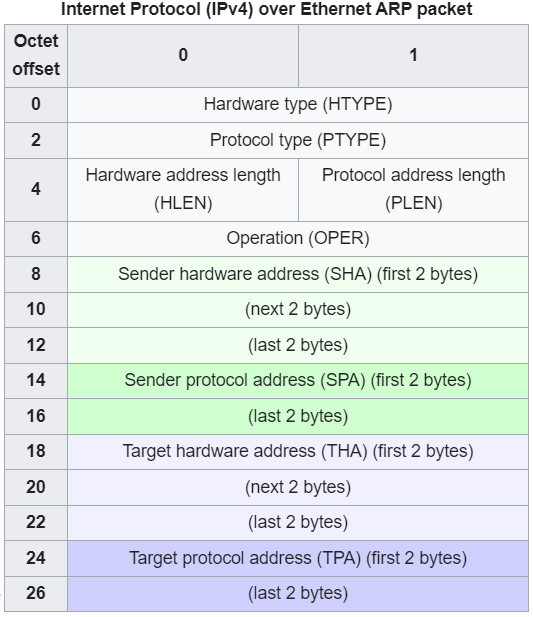
\includegraphics[width=0.6\columnwidth]{images/m7-networking-arppacket.png}
    \caption{Layout of an ARP packet. \cite{wikipedia}}
    \label{figure:arp-packet}
\end{figure}
A more complete ARP protocol implementation involves more functionalities such as probes, announcements, etc. For the purposes of this milestone, only MAC address discovery was implemented. This only requires two message types:
\begin{itemize}
    \item \textbf{ARP request}: machine \textbf{A} does not know machine \textbf{B}'s MAC address, so in its ARP packet it fills in a special \textit{broadcast} destination MAC address of FF:FF:FF:FF:FF:FF. All machines in the local network will receive this packet, and by the protocol only the machine with the destination IP address must respond with a reply.
    \item \textbf{ARP reply}: machine \textbf{B} sends back an ARP packet through the local network with the source and destination fields inverted, with the exception of what is now the source MAC address. Instead of the broadcast address, it fills in its MAC address to be sent back to the requesting machine.
\end{itemize}
Caching of ARP requests and replies was also implemented. This was relatively simple and involved the use of a hash table, as provided from the \textit{collections} library. If the machine received an ARP request, it would store the source IP $\rightarrow$ source MAC mapping within the cache, as well as sending back the reply. Upon receiving the reply from an initial ARP request, the same thing would be done with the destination IP and MAC address.

\subsection{ICMP Protocol}
The ICMP protocol is a network-layer protocol that is used to send error and other operational information between devices operating at that layer. In this milestone, however, we are only concerned with the implementation of sending ping packets.
\\\\
A ping packet is simply an ICMP packet where the "type" and "code" fields are both 0. When a machine that implements this protocol receives such a packet, it is simply to send back the same packet to its source. There are a few quirks with this protocol that would need to be handled, however, such as the $DF$ flag being set within the IPv4 header. This flag states that the overall packet being received is too large for the underlying network hardware to take in as a single packet, and it must be fragmented. Normally, a network stack would be responsible for re-assembling the packet, but this is not required for the purposes of this project. This ICMP protocol implementation is simply to drop such a packet.
\\\\
An important part of implementing the IP protocol is error-checking. This is implemented by a simple checksum algorithm which takes the one's complement sum of all the IP header words, then takes the one's complement of this resulting value. Upon reception of a packet containing an IP header, this checksum is checked against the entire header - if the value is not what is expected, the network stack is to interpret this as an error and drop the packet. For this project, a simple function was available to use to calculate the checksum.

\subsection{UDP Echo Server}
This part of the milestone involves setting up a simple echo server using UDP with a hard-coded port. There is not much design to be had here, as the implementation (had I carried it out) is rather prescriptive.
\\\\
With a working ping functionality from the previous part, a process would then be setup to be running in an infinite loop, which keeps attempting to receive packets. Upon reception, it would simply hand the packet off to the network stack to be processed, as was described previously. In the case of the echo server, a received ping packet would result in an identical packet being sent back to the source IP and port over UDP.

\subsection{Multiple Clients}
This part of the milestone involves setting up a generalized networking service which other processes within the OS can use. For our OS, the API would be an RPC interface. Each RPC call would call upon a particular function within the stack that would carry out a particular protocol, as discussed previously. However, the question is then this: how exactly is the underlying driver running that the network stack is passing its data down to?

\subsubsection{Possible Designs}
One possible way in which the driver could run is directly within the \textit{init} process. This is a design that we had used for milestone 4 and onwards, mostly because of its simplicity. This special process has certain capabilities already set up for us that makes starting a service within it much easier, and the same is true for the network driver - the device frame capability is directly exposed to the driver, and it can just use it. The existing RPC bindings to \textit{init} can also be used, and not much additional setup to expose this service would be required. However, there is the downside of performance with this approach, especially because of the fact that we already have multiple services (memory management, process management, etc.) that \textit{init} is running.
\\\\
On the contrary, the performance gains from running the driver in its own process is clear, as that process would only be responsible for serving RPC requests for networking functionalities. With this design, however, other processes must then know how to bind to this one in order to be able to make such calls in the first place. Our binding interface that was fleshed out to handle UMP as well as LMP in milestone 6 is capable of this, but only between a process and \textit{init}. We would need to be able to carry out arbitrary bindings between two processes, of which one way this could be achieved is with a working name server. The networking server would register itself with the name server, and other processes would be able to query this name server to get a binding to the networking server.

\subsection{Challenges}
This milestone was particularly challenging due to environment setup issues. With only minor modifications required to given build files associated with this project (that took me a long time to realize), there was still an issue with how I had been running QEMU. I had been using WSL2, which is essentially a Linux VM running within my host Windows 11 OS, and this VM is then running QEMU. With a lot of investigation, I came to the conclusion that it's not possible (or at least I won't figure it out in a reasonable amount of time) to send packets from the OS running within QEMU, which has to make it past whatever virtual network interface(s) there is/are at the QEMU - Linux boundary, and then past the Windows - WSL boundary. With a WireShark instance running inside WSL, I can see that packets successfully make their way outside of QEMU, but no such packets ever make it outside of WSL. As a result, the only way in which I was able to test my code was to send packets to a network interface within WSL itself, which had its own quirks in and of itself (such as a dynamically-changing MAC address).
\\\\
There is also a challenge unique to debugging networking implementations, and that is stray packets being received that you do not expect. At first, they appear to be packets that you intended to receive based on what was just sent, but one then may realize that other packets from mostly-unknown sources can be randomly sent at any time. In order to combat this, reception just has to run for long enough to make sure there was ample time for the expected packets to arrive, and to ignore other packets. Naturally, this lends itself to the strategy of simply dropping and packets the network stack does not know how to handle.
\newpage

\section{Capabilities, Revisited}
For the final Milestone, each group member was required to individually implement different Barrelfish subsystems and then jointly integrate them at the end. This chapter delves into \textit{capabilities} and was completed by \textbf{Arya}.

\subsection{Introduction}
To fully leverage the power of Barrelfish's capability system, some additional capability operations needed to be implemented. 
\\\\
First, adding the ability to share capabilities across cores allows for more powerful communication between them. Proper tracking of shared capabilities increases the safety of services that hand out capabilities to the other core, like the memory server.
\\\\
Additionally, \texttt{delete}, \texttt{revoke}, and \texttt{retype} operations are always sent first to the kernel through a system call, but there are some situations where the kernel is not properly able to handle the request, and instead leaves the responsibility to the monitor. Some of these situations are as follows:
\\
\begin{itemize}
    \item \textbf{Deleting a CNode or Dispatcher capability}: These types of capabilities contain additional capability slots within them. The internal capabilities need to be deleted as well, but this will take multiple steps, and in keeping with the microkernel architecture, the kernal should not perform a long-running operation like this. 
    \item \textbf{Revoking a capability}: Similarly, the kernel should not revoke a capability, because doing so could involve many delete steps (eg. deleting a number of descendants).
    \item \textbf{Deleting the last copy of a shared capability}: If a capability is shared between cores, the monitor needs to negotiate the deletion.
    \item \textbf{Revoking a shared capability}: Similarly, when revoking a shared capability, the monitor needs to ensure that the capability is revoked over the entire system.
    \item \textbf{Retyping a shared capability}: To maintain capability invariants, the monitor needs to check with the remote core as well as the local one to ensure a retype operation is legal.
    \item \textbf{Deleting the last copy of a mem-backed capability}: When the last copy of a capability that refers to physical memory is deleted, the monitor is invoked so that it can notify the memory manager and thus free the resource for future allocation.
\end{itemize}
\subsection{Handling Operations in the Monitor}
\noindent
When system capability operations fail with the error code \texttt{SYS\_ERR\_RETRY\_THROUGH\_MONITOR}, the child process sends an LMP message to its local monitor containing its root CNode, and the address of the relevant capability. The monitor is able to complete the operation on the capability, even though it is from a different CSpace, by referring to the child dispatcher's root CNode.
\\\\
Some operations are sent to the monitor because they would take too long for a single syscall. This occurs when deleting a CNode or Dispatcher capability, or when revoking a capability. The monitor first marks all relevant capabilities for deletion, which creates a queue of delete steps. Each delete step can be completed as a single syscall, and the monitor iterates through the delete steps until all are completed. Once complete, it sends an LMP acknowledgement to the child to indicate that the process has completed. \\
This way, each syscall completes in a bounded time, which is one of the invariants necessary for a stateless kernel.

\subsection{Distributed Capabilities}

Some precautions need to be taken for distributed capabilities to ensure a safe system state. Every capability has a specified owning core, every copy of the same capabilities must have the same specified owner, and the owning core must always have a copy of all capabilities it owns. The first step of ensuring these invariants happens when a capability is shared between cores.
\\\\
To share a capability with another core, a process sends a request to its local monitor (if it is not already the monitor). While the monitor can identify and perform operations on capabilities in a child process' CSpace by referring to the child's root CNode, it cannot do this for capabilities on another core. For that reason, whenever a capability is going to be transferred cross-core, the monitor generates a unique key for it, and stores the key and capability in a hash table. It sends the capability information to the other core along with the generated key, and the other core's monitor creates a local copy of the capability and stores it with the shared key in its own hashtable.
\\\\
The monitors both set the same owner of the capability as specified in the transfer message, and set each capability's remote relations metadata to indicate that they have a remote copy. As a result, the kernel will pass certain operations (like deleting the last copy on this core) up to the monitor to handle.
\\\\
For any cross-core operations involving shared capabilities, the cores can communicate efficiently using the shared key of the capability (see Figure \ref{figure:m7_shared_key}).

\begin{figure}[ht]
    \centering
    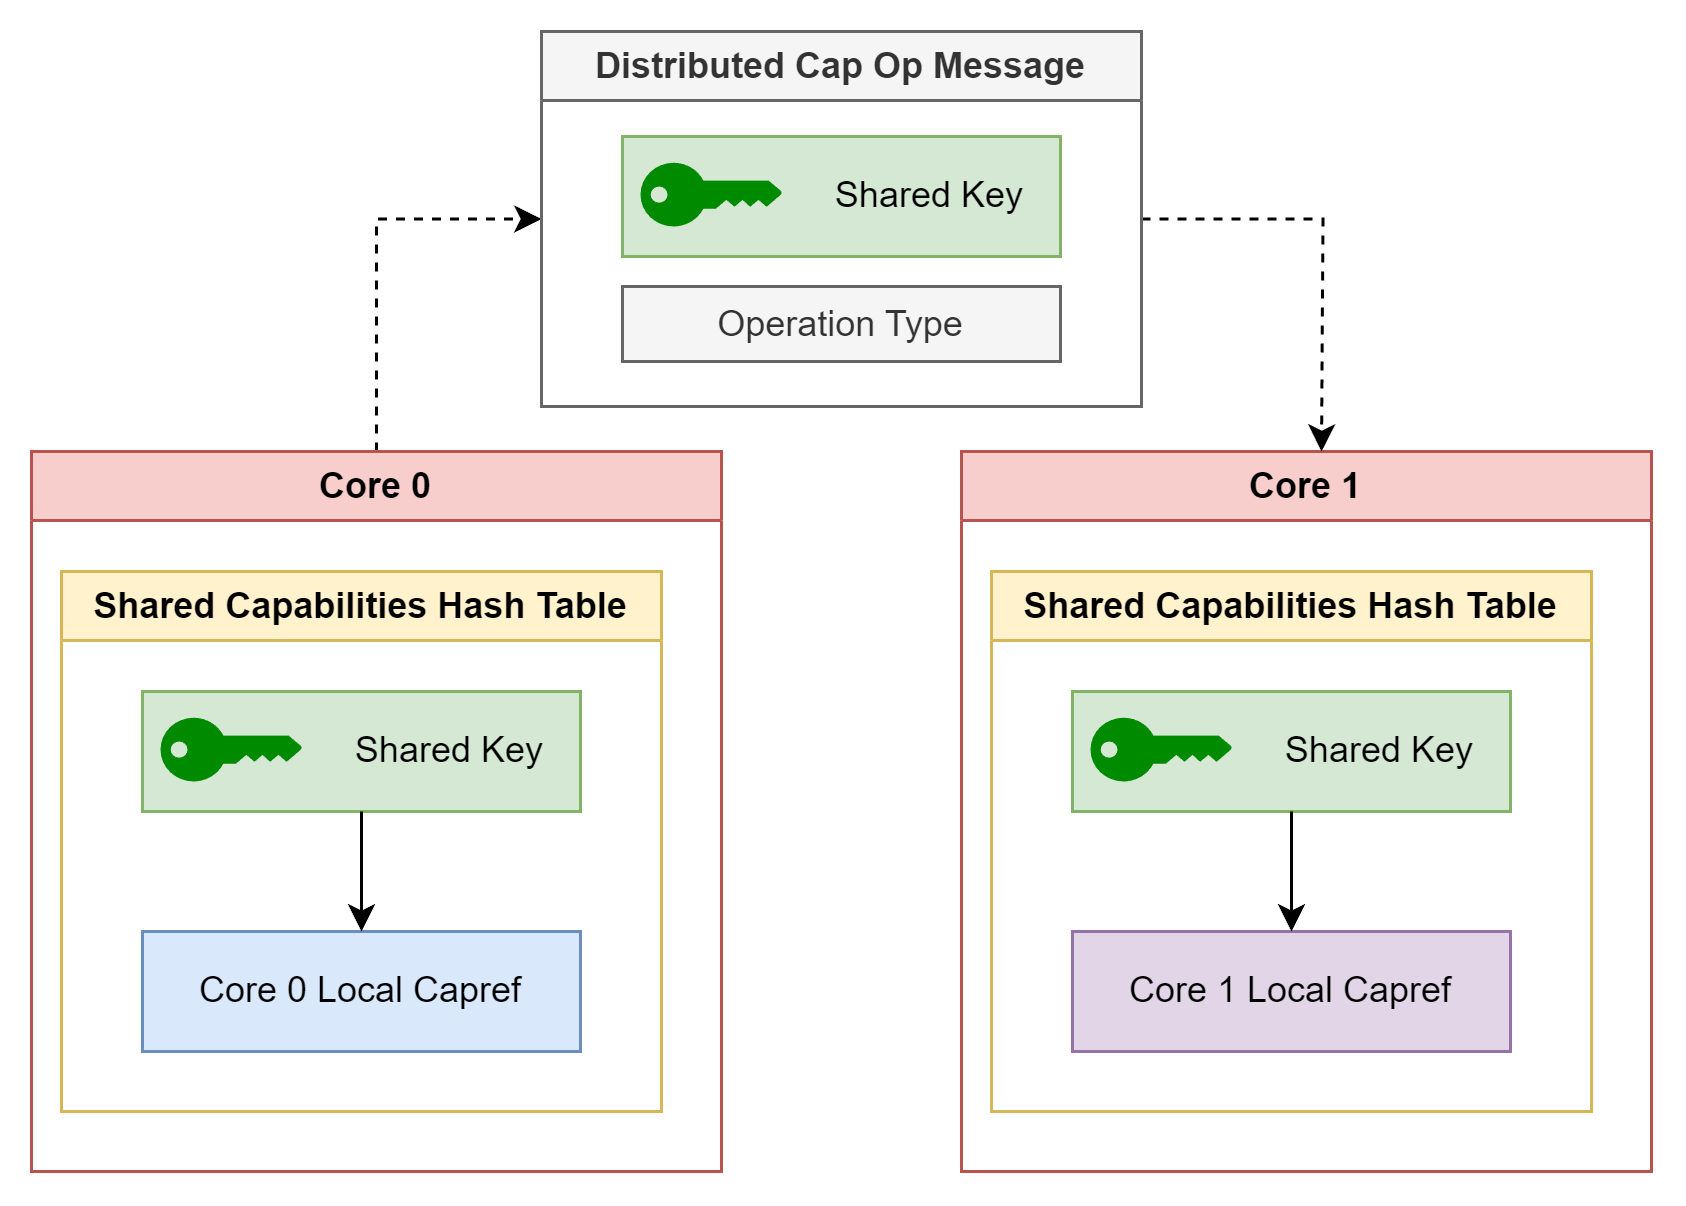
\includegraphics[width=0.8\columnwidth]{images/capability_ops.png}
    \caption{Cross-core capability operations using a shared key}
    \label{figure:m7_shared_key}
\end{figure}

\subsection{Coordinating Distributed Operations}

\textbf{Deletion}: 
When the last local copy of a shared capability is deleted, the local monitor is notified. There are three potential cases: \\
\begin{enumerate}
    \item If the capability is owned by the local core and ownership is transferable, the monitor sends a \texttt{TRANSFER\_OWNERSHIP} message to the remote core, then deletes its local copy. Once the remote core acknowledges the transfer of ownership, the deletion is complete.
    \item If the capability is owned by the local core but the capability type cannot have its ownership transferred (eg. a dispatcher capability), then the remote core is sent a \texttt{DELETE\_ALL} message notifying it to delete its local capabilities. When the remote core acknowledges completion, the deletion is complete.
    \item If the capability is not owned by this core, the monitor sends a \texttt{NOTIFY\_DELETED} message to the other core. This step is not strictly necessary, but it allows the other core to delete any metadata for the capability that is no longer needed (eg. in the shared capability hashtable), and to update the remote relations of the capability.
\end{enumerate}
\\
\textbf{Revocation}: Revocation of a capability should ensure that no copies or descendants exist in the entire system, not only in the local core. When a shared capability is revoked, regardless of which core owns the capability, the other core needs to be notified to delete any copies and descendants. The monitor marks its local copies and descendants for deletion, then sends \texttt{DELETE\_ALL} message to the other core. The other core marks and deletes its own copies and descendants, then replies with a \texttt{DELETE\_SWEEP} message, triggering the original core to complete its local delete steps and complete the operation.
\\\\
\textbf{Retyping}: Retype operations are illegal in certain situations, such as when another descendant already exists. For consistency, this invariant must be maintained system-wide, not only on the local core. When a retype operation is invoked on a shared capability, the operation is sent to the monitor. The monitor sends a \texttt{CAN\_RETYPE} message to the other core. The other core checks for local descendants of the shared capability, and responds YES or NO. If YES, the local monitor can successfully perform the retype operation. If NO, the operation fails because it is not a legal retype.

\subsection{Shared Capabilities and Concurrency}

The shared capability operations present some issues if used concurrently. To help mitigate this, the monitor is able to "lock" a capability to indicate that no other concurrent operation should be performed on it. For example the monitor locks a capability when trying to perform a retype on it, and also locks the capability when the remote core requests to check if the capability can be retyped. This prevents the monitor from providing inconsistent answers (eg. it tells the other core that it can retype the shared capability, while simultaneously retyping the capability locally).
However, it is a difficult task to ensure that no conflicting operations ever occur. If designing an OS for deployment, each possible concurrent operation would have to be considered. Barrelfish implements a "Two-Phase-Commit" protocol to better guard against inconsistencies due to concurrency, but this would have been too complicated to implement in the given time.

\subsection{Memory Server Integration}
The memory server was first introduced in M4, but it was revisited during this milestone because it was modified to use the safe capability sharing operations. This modification also unearthed some existing issues with the memory server implementation.
\\\\
\textbf{Memory Distribution}:
We chose to implement core 0 as the main memory server, so that most memory would be consolidated in one place, and core 1 is able to request more memory as necessary. An advantage of this approach is that memory only needs to be requested in one direction, preventing potential complications of both cores requesting memory from eachother. A disadvantage is that the overhead of memory operations is increased when core 1 needs a lot of memory. If the OS were to be used for a particular workload where the programmer was aware of where memory would be needed most, they might choose to implement this differently to optimize memory access.
\\\\
The monitor on core 1 can request RAM capabilities from core 0, and child processes on either core and request RAM from their local monitor. When child processes request memory from core 1's monitor, it forwards the request to core 0.
\\\\
\textbf{Sharing Memory with Distributed Capabilities}:
A benefit of the distributed capabilities system is it allows for a better memory server implementation. Previously, when requesting RAM from the other core, the unsafe \texttt{ram\_forge} operation was necessary to create a RAM cap on the receiving core. Now, the capability is sent safely, and the ownership is transferred to the receiving core. This choice was made so that the memory server does not need to keep a copy of the RAM, and the child process does not need to invoke the monitor constantly when performing local operations on the received RAM. Only when the last copy of the memory is deleted on the receiving core, and operation is sent to the monitor, does the monitor sends a RAM capability back to the memory server to free. In fact, any cap that is backed by physical memory will trigger the memory to be freed automatically when the last copy of the capability is deleted. This is a powerful effect of the capability system, and ensures that memory leaks do not occur as long as capabilities are cleaned up correctly.
\\\\
\textbf{Coordinating Remote RAM Requests}:
Coordinating processes to correctly request remote RAM proved to be more difficult than expected. The crux of the issue was that sending and receiving an RPC call requires RAM itself, so a process/core cannot wait until it is out of memory to request more. This issue is reminiscent of the memory threshold for Memory Manager in M1. However, there is more difficulty here because child processes do not have a memory manager; they begin with a capability to some initial starting memory, then any additional memory needs to be requested from the memory server. There is no way to "refill" and manage the starting memory. For this, we would need to initialize a memory manager in every dispatcher, and refill it with memory from a monitor.
\\\\
To prevent infinite loops, we implemented a flag that prevents a process from requesting remote memory while it is in the process of requesting remote memory, or while servicing a page fault. This imposes severe limitations on the memory sharing system. Each dispatcher starts with a fixed amount of "starting memory", and it requests remote RAM to serve allocation requests whenever possible, but falls back on the starting memory in the indicated situations. This means that a dispatcher will eventually run out of memory, even when there may be plenty of additional memory in the monitor.
\\\\
\textbf{Alternate Sharing Designs}: 
There are several other ways that RAM capabilities might be shared between cores.
\begin{itemize}
    \item Initially, we considered the possibility that the memory server's core maintains ownership of sent capabilities. However, this would cause additional overhead in the form of metadata (shared capabilities in the monitors' hash tables), and more capability operations on the receiving core would trigger the monitor. The idea was abandoned for this reason.
    \item Another option, as mentioned earlier, would be for each dispatcher to have its own memory manager. When the memory available falls below a certain threshold, it would request a large chunk of memory to add. This has the advantage of reducing the number of RPC calls in the system and preventing dispatchers from prematurely running out of memory. A disadvantage is that this could cause greater memory fragmentation, since dispatchers would be holding large chunks of memory which may not be freed for a long period of time (or until the process exits). This design seems promising, but it would introduce additional complexity, and the memory manager was not designed to be used outside of the monitor. We chose not to take the risk of doing so now.
\end{itemize}
\subsection{Challenges}
A particular challenge with this milestone was "filling in the blanks" of the monitor with respect to the underlying kernel code. In some cases it became apparent that the kernel code for capability operations was made for a different monitor design. In some cases I modified the checks in order to pass operations up to the monitor that previously would not have been, because my design required it. For example, I modified the kernel code to pass retype operations up to the monitor for any capability with remote copies, not only remote descendants. This was necessary since, in my implementation, a monitor will not necessarily be notified when the other core does a local retype, so it will not know that the capability has remote descendants. My solution was to always pass the retype operation for shared capabilities up to the monitor so that the monitor can query the other core for descendants.

\subsection{Conclusion}
The completed deliverables are all demonstrated in the \texttt{capabilities\_m7} binary, which expects to be run on core 1 so that it gets RAM capabilities from the remote core. The implemented functionalities are:
\begin{itemize}
    \item The monitor can receive and process capability operations.
    \item \texttt{cap\_revoke} and \texttt{cap\_delete} work on a single core for any capability.
    \item Can send capabilities cross core over UMP with the right remote relations (I did not implement spawn with caps cross core, but used a \texttt{send\_cap\_remote} RPC call to test the functionality).
    \item Handle \texttt{cap\_delete}, \texttt{cap\_revoke}, \texttt{cap\_retype} for any capability including ownership transfer and remote relations.
    \item Use the capability transfer mechanism cross core in the memory allocation system.
    \item Return no-longer used memory back to the memory server.
\end{itemize}

\newpage

\section{Shell}
For the final Milestone, each group member was required to individually implement different Barrelfish subsystems and then jointly integrate them at the end. This chapter delves into the \textit{shell} and was completed by \textbf{Linh}.

\subsection{Introduction}
We have a somewhat fully functioning operating system up to this point. However, to do anything with it, we'd have to shut it down, add some user code, hook that code statically into the system code, re-start the system. Then, it finally carries out whatever task we wanted to do. What if we don't want our system to run this code every time it starts? What if we simply wanted to access some resource without needing to write and compile code for it? It is also a bit silly to have to shut down the entire system in order to do any sort of dynamic task. The solution to all this is to implement a shell, which allows real-time user interaction with the system.

\subsection{Enabling User Input}
The serial device that we use to read input from a user's keyboard is the PrimeCell UART (PL011).  In Barrelfish, the driver for this runs in user-space, and is set up by mapping a frame containing the register regions into the domain where the driver will run. Although our \texttt{init} process is becoming monolithic at this point, it is still the simplest method of running this driver. So, the frame containing the register regions for the PL011 is mapped into \texttt{init} and is also where the driver runs. With this set up, processes can now access the serial driver via the RPC library to read user input or to write to the driver's output. 


\subsection{Coordinating the Shell with \texttt{init}'s Other Responsibilities}
Recall that in Milestone 6, we decided to have \texttt{init} function as all resource servers until the nameservers were implemented. At the time of implementing the shell, the nameserver functionality was not yet complete, and so \texttt{init} still must handle all RPCs. The shell must wait for user input in order to perform any operation, and this ``waiting" cannot block \texttt{init}'s other responsibilities. This is done via device interrupts and using a separate thread to handle all commands invoked through the shell. 


In Milestone 6, we had created a separate waitset for each RPC channel, and a separate thread for each of them, waiting to dispatch events. In order to not interfere with the handling of these events, the shell receives interrupts from the UART driver on its own LMP channel, in which there is a separate thread that waits on these interrupts and handles them in sequence. So, at any given time in \texttt{init}, there may be multiple threads waiting on its own waitset for either servicing an RPC call, or a user-given shell command (See Figure \ref{figure:m7-shell-threads}). It was particularly important to use device interrupts to retrieve user-input, since the shell is running in \texttt{init}. Polling the device for user-input would've been extremely wasteful usage of \texttt{init}'s resources, and would slow down RPC messaging as a whole. With this layout, the shell should never block any other activity occurring in the system.  

\begin{figure}[ht]
    \centering
    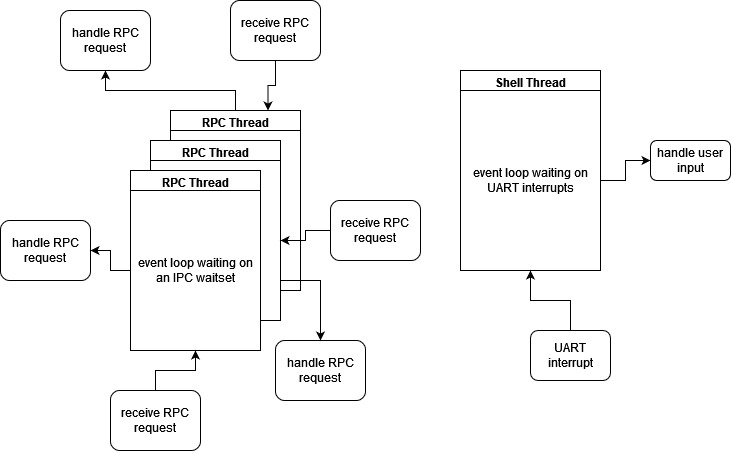
\includegraphics[width=0.8\columnwidth]{images/m7-shell-threads.jpg}
    \caption{The many threads running in \texttt{init} at any given time}
    \label{figure:m7-shell-threads}
\end{figure}

\subsection{Shell Commands}
It was pretty straightforward to implement the various commands the user can enter into the shell, since most of the functionality already existed, it just needed to be called. There is much not design required for this. The general sequence of events that occur during command execution are: 

\begin{enumerate}
    \item Receive user input
    \item Buffer the user input until a newline character is entered
    \item Upon receiving a newline, interpret the buffered input as a command (and perform the appropriate argument verification)
    \item Handle the command synchronously using pre-existing functionality by simply calling it
    \item If the command is meant to happen asynchronously, create a new thread to execute it. Store any required state upon the thread exiting.
\end{enumerate}

The full list of supported commands are:

\begin{itemize}
    \item \texttt{echo [string] ...} - prints out the given string of characters 
    \item \texttt{run\_memtest [n]} - allocates n bytes of memory, then tries to write and read them
    \item \texttt{run [cmdline] [\&]} - runs an application with the given commandline, will be in background if ``\&" is provided
    \item \texttt{oncore [coreid] [cmdline] [\&]} - same as ``run", however allows specification of which core to run on
    \item \texttt{ps} - lists out active running processes
    \item \texttt{kill [pid]} - kills the process with the given pid
    \item \texttt{help} - lists all available commands
    \item \texttt{ls} - lists the current files and directories in the current directory
    \item \texttt{mkdir [path]} - create a new directory at the given path
    \item \texttt{rmdir [path]} - removes a directory at the given path
    \item \texttt{cat [path]} - dumps the contents of the file at the given path
    \item \texttt{rm [path]} - removes the file at the given path
    \item \texttt{time [command]} - prints the time taken to execute the command in microseconds
\end{itemize}

\subsubsection{A ``Fake" Filesystem}
A core functionality to any shell is to expose the filesystem to the user. However, we unfortunately did not have a real one, and the filesystem related commands, \texttt{ls, mkdir, rmdir, cat, rm}, were implemented with the provided \texttt{RAMFS} library. The commands only work on ``temporary" files and directories, which exist only during the run-time of the system since there is no persistent file system available to save them to. In order to demonstrate the \texttt{cat} command, a temporary text file was created upon system startup simply for the purposes of calling \texttt{cat} upon it.

\subsubsection{Process Management Through the Shell}\label{m7-shell-pm}
Another core functionality of a shell is to allow the user to arbitrarily run any application they wish. Our current OS isn't quite there yet, since we don't have a filesystem. The user can run any application that has been compiled in one of the multiboot images that are ``hardcoded" into our OS.  
The \texttt{run} and \texttt{oncore} commands allow for this, and require some process management. In order to capture the exit code of a process to support the \texttt{\$?} variable, upon handling one of these commands, the shell must wait for the process to exit. Luckily, this was previously implemented in Milestone 4. However, unluckily, it was intended to be called through RPCs by processes \textit{other than} the process management server. 
%, when the user enters \texttt{run hello}, for instance, to start a process in the foreground, the shell-handling thread in \texttt{init} must wait for the \texttt{hello} process to exit. 

Due to our \texttt{init} process becoming a monolith that now includes the shell and the process manager, this required slightly adapting the process management functions to allow \texttt{init}'s shell-handling thread to wait on a process. At a high-level, this is done through waitsets, in which the shell creates a separate waitset for waiting on processes to exit. If the process is run in the foreground, waiting on this waitset is done in the same thread as the one which waits on the UART interrupts so as to allow the user-given process to ``consume" the shell console (Refer to Figure \ref{figure:m7-shell-proc-wait}). If the process is run in the background, a separate thread is created to wait on it to exit, allowing the shell-handling thread to continue to receive user input. 

\begin{figure}[ht]
    \centering
    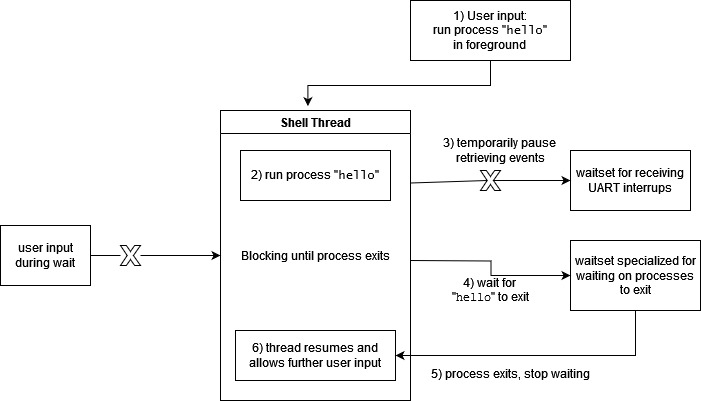
\includegraphics[width=0.8\columnwidth]{images/m7-shell-proc-wait.jpg}
    \caption{The shell thread running a foreground process}
    \label{figure:m7-shell-proc-wait}
\end{figure}

\subsection{Alternatives: Using a Separate Process for the Shell}
A more sophisticated approach to running the UART driver, and the shell, would've been to create a separate process that acted as the terminal server. The primary reasons in which this approach was not taken are:

\begin{itemize}
    \item It is much simpler to not have to set up an entirely separate process for the shell, which would require \texttt{init} to know about this server and keep track of it somewhere to allow other processes to bind to it. Furthermore, we would need to move the RPC handlers (which currently live in \texttt{init}) for writing and reading from the serial driver into this process, and ensure that it can receive requests from other processes. This is not particularly complicated, however, it does require some shifting around of code and can introduce a lot of unexpected problems that we didn't have time to deal with.
    \item In anticipation for the completed nameserver, we felt that it would be wasted effort to try to set up the terminal server in a rudimentary way before a proper nameservice binding mechanism was in place. However, since the nameserver ended up not completed, the shell ended up never migrating to its own process.
\end{itemize}

Although running the shell in \texttt{init} is easier and can work for simple use cases, it is not very good design for a system pushed out to production. The process management described in Section \ref{m7-shell-pm} highly coupled the shell's code with that of the process manager. The shell must deal with waitsets and closures, that are normally fully abstracted away from the client during an RPC. However, this coupling is inevitable due to the fact that the process manager itself is not meant to be waiting on processes to exit. To further develop the shell on top of this would definitely require de-coupling the two by moving the shell into a separate process.




\newpage

\section{Nameserver}
For the final Milestone, each group member was required to individually implement different Barrelfish subsystems and then jointly integrate them at the end. This chapter delves into the \textit{nameserver} and was completed by \textbf{Mathew}.
\\\\
Due to time constraints I was not able to get this Milestone done, so this chapter is written from a ``what if" perspective. All design here is theoretical and may gloss over some finer details that only would have been revealed during the implementation process.

\subsection{Introduction}
Up until this point, we have been writing services for our operating system that are hardcoded into the RPC library. For example, in order for a user process to communicate with the process management server, it needs to make a call to \texttt{aos\_rpc\_get\_process\_channel}. If it wants to get the status of a process, it then needs to make a call to \texttt{aos\_rpc\_proc\_get\_status}. This is not sustainable and somewhat antithetical to the idea of the microkernel, so we set out in this chapter to implement a ``nameserver". The nameserver, in theory, acts as a mediator between clients and services. For example, a service should be able to register itself under a unique name with the nameserver, and a client should then be able to query the nameserver and receive a handle for communicating with the service.

\subsection{Design Constraints}
The nameserver will have to handle a steady amount of requests over time since it is possible for hundreds of processes to simultaneously be running on our operating system. We can expect a fair amount of these processes to make at least one or two requests to the nameserver so as to either register a service or look one up. On that note, we also want to think about how the nameserver should structure its data since it must hold mappings between registered service names and their connection data. I identified the following challenges with respect to the nameserver implementation:
\begin{itemize}[itemsep=0pt]
    \item How does binding work? The nameserver needs to do some routing so that an arbitrary client and service can connect to each other.
    \item How should the nameserver store its service data?
    \item Which services should the nameserver return when responding to a search request?
    \item How does a service deal with multiple client connections?
    \item Should the nameserver run on the monitor or in its own process?
    \item How do nameservers on different cores coordinate with each other?
\end{itemize}

\subsection{Possible Implementations}
We need to start off by thinking about where the nameserver will \textit{live}. Assuming that we want to use UMP for binding requests (which would be ideal since it's faster than LMP), the monitor will somehow have to be involved in order to transfer capabilities across cores. This leaves us with two options, the first being to simply run all nameserver functionality on the monitor (Figure \ref{figure:nameserver}). RPCs to the nameserver in this case would require a minimal amount of IPC and the implementation effort would be straightforward, but the design is less faithful to the Single Responsibility Principle.
\begin{figure}[ht]
    \centering
    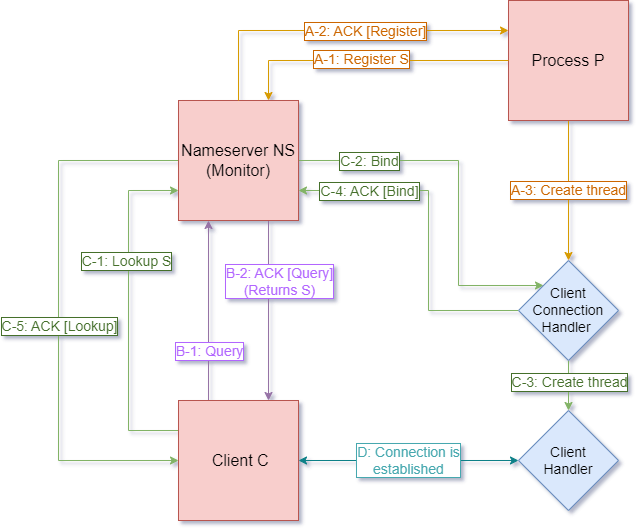
\includegraphics[width=0.5\columnwidth]{images/nameserver.png}
    \caption{Call graph for a nameserver running on the monitor.}
    \label{figure:nameserver}
\end{figure}
\\\\
The second option involves distinguishing between \textit{naming} and \textit{binding} (Figure \ref{figure:bindingserver}). In this case, the nameserver runs in its own process and stores a mapping between service names and their channels. The ``binding server" is the monitor, and is communicated with whenever the nameserver needs to create a connection (either between itself and a service, or between a client and a service). This approach is nice because not all cases where processes want to bind with each other make sense as a ``service". In these cases, they simply make an RPC to the binding service and don't have to worry about advertising themselves to the nameserver. This separation of concerns adds some overhead however, as more RPCs are necessary for the nameserver to handle binding. 
\begin{figure}[ht]
    \centering
    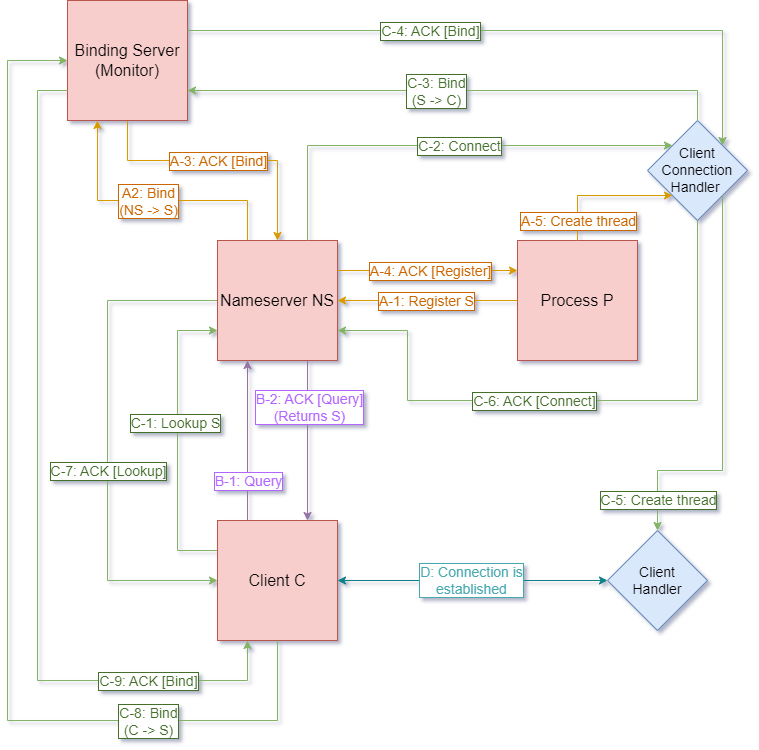
\includegraphics[width=0.5\columnwidth]{images/bindingserver.png}
    \caption{Call graph for a nameserver running outside of the monitor.}
    \label{figure:bindingserver}
\end{figure}
\\\\
As mentioned previously I did not actually implement anything, so in the spirit of taking the easier approach we assume the nameserver runs on the monitor (option 1) for the rest of this chapter. Also assume that like before, all new processes spawn with a connection to the monitor (running the nameserver). This is the only connection necessary since all other services can be accessed using it.

\subsubsection{Registration}
A process \textbf{P} registers a service \textbf{S} with the nameserver \textbf{NS}:
\begin{enumerate}[itemsep=0pt]
    \item \textbf{P} sends a \texttt{register} request to \textbf{NS} containing an identifier for \textbf{S}, and a UMP/LMP capability to itself.
    \item \textbf{NS} creates a connection to \textbf{P} using the capability, stores a mapping between \textbf{S} and the connection, and returns an ACK.
    \item \textbf{P} creates its side of the connection and spawns a thread to listen on it. The thread is set up with a message handler that handles new client connection requests. We will refer to this thread as the ``client connection handler" (\textbf{CCH}).
    \item \textbf{P} stores a mapping between the service handler (the function that will be used to respond to clients) and the identifier for \textbf{S}. This handler will run on a thread when a new client connects. We can expect \textbf{P} to run a small number of services, so a linked list will suffice here. A hash table would be marginally faster (on average), but I figured that if I were to have completed this Milestone, I would have saved myself the headache.
\end{enumerate}
Note that under this scheme, one process may run multiple services (each service having its own connection handler thread). Also note that the client connection handler allows a service to serve multiple clients (this is explained in detail later).

\subsubsection{Queries}
When a client wants to ``search" for registered services, it makes an \texttt{enumerate} request to the nameserver. This breaks down into two problems: what data structure does the nameserver use to store service mappings, and what string-searching algorithm does it implement to find those mappings when queried? The search problem also ties in with naming, since it depends on what exactly processes provide as a name when registering a service. It would be a bit overkill at this point to introduce sophisticated naming/search schemes since we only have a few services running, so for now we assume that names may only consist of alphanumeric characters, and that queries return all names containing the search string as a subset. More formally, given a set of names $N$ and a search string $s$, we return all names $n \in N$ such that $s \subseteq n$.
\\\\
The string-search algorithm we implement places limitations on how mappings are stored. A hash table would be very nice here since it fits our need of quick lookups, insertions, and deletions, however using one necessitates that when queried we only return names that exactly match the search string. This would effectively turn \texttt{enumerate} into a ``service exists?" request, which is less than ideal. Instead, we opt for a linked list. Registrations become constant-time (we can just insert at the front/back), while deletions/lookups suffer a bit and turn into linear-time operations, since we have to search the list for anything matching our search string. A case can be made that this is fine since we're not expecting a massive number of services, however an analysis of the ``average case" would be needed to back that claim, and linked lists don't mesh too well with cache/memory since each access requires a pointer-hop. While thinking about this I realized that an abstract syntax tree would solve some of these issues, however I figured that I ultimately would have went with the linked list due to its simplicity.

\subsubsection{Lookup}
A client \textbf{C} asks the nameserver \textbf{NS} for a connection to a service \textbf{S} (running on \textbf{P}):
\begin{enumerate}[itemsep=0pt]
    \item \textbf{C} sends a \texttt{lookup} request to \textbf{NS} containing the name of \textbf{S}, and a UMP/LMP capability to itself.
    \item \textbf{NS} sends a ``bind`` request to \textbf{S}, which is caught by its client connection handler \textbf{CCH}.
    \item \textbf{CCH} creates its side of the connection and spawns a thread \textbf{CH} to listen on it. The thread is set up to run the service handler that \textbf{P} stored during the registration process.
    \item \textbf{CCH} returns an ACK to \textbf{NS}, which returns an ACK to \textbf{C}.
    \item \textbf{C} creates its side of the connection and can now talk with \textbf{P}. Requests from \textbf{C} are caught and responded to by \textbf{CH}. 
\end{enumerate}

\subsection{Multicore Support}
The final issue we have to deal with is multicore support. Since each core has its own monitor, and the nameserver \textit{is} the monitor, we need a way to synchronize their service lists. When a service registers with the nameserver, we need to decide if we want to notify the other core immediately, or hold off until a request comes in that requires the aggregate list (e.g. \texttt{enumerate}). Ideally, we want to pick a design that minimizes the amount of IPC happening.
\\\\
If we decide \textit{not to notify} the other core immediately, the nameserver needs to query it before serving \texttt{enumerate}, \texttt{lookup}, and \texttt{deregister} requests. \texttt{enumerate} is relatively easy to implement since we just have to make another \texttt{enumerate} request to the other core and then concatenate the list before serving the request. \texttt{lookup} also requires us to make an \texttt{enumerate} request to the other core, if the nameserver serving the request does not find the service in its local list. If it doesn't, it must make a cross-core binding request (we have an implementation for this from Milestone 6). Finally, \texttt{deregistration} under this design requires cross-core calls no matter what. Since services may be distributed (e.g. process management), the nameserver needs to make another \texttt{deregister} call to the other core. Similar to Milestone 6, we need to be careful about infinite loops in \texttt{enumerate} and \texttt{deregister} since these calls get propagated to the sister core (setting a flag in the request works here).
\\\\
If we decide \textit{to notify} the other core immediately, the nameserver needs to talk to the other core during \texttt{register} and \texttt{deregister} requests. I would have chosen this design because we can always expect exactly 1 \texttt{register} and 1 \texttt{deregister} to happen per service, but we can't be sure how many \texttt{lookup} and \texttt{enumerate} requests might happen for a given client (which are less costly operations using this design). With this design, note that the nameserver must know what core its stored services are on in order for \texttt{deregister} and \texttt{lookup} to work (so that it knows whether or not to forward these calls).

\newpage

\section{Conclusion}
\subsection{Summary}
It has been a long and arduous journey to get here, but we have now sucessfully implemented a memory allocator (Milestone 1), enabled user-space virtual memory management and paging (Milestone 2), spawned new processes (Milestone 3), booted additional cores (Milestone 5), and have a mechanism to allow processes across cores to communicate (Milestones 4 and 6). In Milestone 7 we extended our system to have more specialized features such as networking, a more advanced capability management system, a shell, and a nameserver.  

\subsection{Outcomes}
The project provided an opportunity to improve both technical and non-technical skills for all group members.
\begin{itemize}
    \item \textbf{Understanding microkernel architecture}:
    We entered this class under the expectation that we'd be taught how the Linux kernel works, as it is currently the standard in most parts of industry and academia. It was a bit of a surprise to be shown a more modern system architecture, which moved away from the monolithic kernel. It was overwhelming at the beginning having to both grasp completely new concepts (which fly in the face of all the ones we're used to), \textit{and} implement them at the same time. Ultimately, we are incredibly appreciative to have been given the opportunity to explore modern kernel design, as it is likely to benefit us when we move into the industry or higher levels of academia. 
    \item \textbf{Organizing group work}:
    All of us had previously experienced group work in a co-op setting, so this was not really foreign to us. However, it was a comparatively smaller codebase that we were working on compared to what we had experienced during co-op, and oftentimes we had to write code on top of each others' in realtime as opposed to things being a bit more isolated. It is much easier to write code than to understand code, and we faced challenges keeping everyone up-to-date on the state of the system while Milestone tasks were being completed. We feel that working in such close conditions allowed us to greatly strengthen our code-comprehension abilities in a short amount of time.
    \item \textbf{Handling a large code base}: Jumping into a system like Barrelfish is initially very daunting due to its many layers and interacting subsystems. It takes skill to determine which parts of the code base are relevant for a particular task and to ensure that subsystems continue to behave as expected by other parts of the code. To make this easier, we ensured that new additions to the code base were as isolated as possible, and used techniques like modular debug messages to keep the logs from becoming overwhelming.
    \item \textbf{Underdefined problems}: Some of the tasks did not describe a particular implementation and allowed us design freedom. Many of these decisions would affect us in later Milestones which exemplified the importance of careful planning. On the other hand, we also learned that spending too much time deliberating on a design can hinder progress. It was beneficial to design with flexibility in mind, so that we could more easily change our architecture in the future if necessary.
\end{itemize}

\newpage

\bibliographystyle{plain}
\bibliography{bibliography}

\end{document}
